%%
%% This is file `mcmthesis-demo.tex',
%% generated with the docstrip utility.
%%
%% The original source files were:
%%
%% mcmthesis.dtx  (with options: `demo')
%%
%% -----------------------------------
%%
%% This is a generated file.
%%
%% Copyright (C)
%%       2010 -- 2015 by Zhaoli Wang
%%       2014 -- 2019 by Liam Huang
%%       2019 -- present by latexstudio.net
%%
%% This work may be distributed and/or modified under the
%% conditions of the LaTeX Project Public License, either version 1.3
%% of this license or (at your option) any later version.
%% The latest version of this license is in
%%   http://www.latex-project.org/lppl.txt
%% and version 1.3 or later is part of all distributions of LaTeX
%% version 2005/12/01 or later.
%%
%% This work has the LPPL maintenance status `maintained'.
%%
%% The Current Maintainer of this work is Liam Huang.
%%
%%
%% This is file `mcmthesis-demo.tex',
%% generated with the docstrip utility.
%%
%% The original source files were:
%%
%% mcmthesis.dtx  (with options: `demo')
%%
%% -----------------------------------
%%
%% This is a generated file.
%%
%% Copyright (C)
%%       2010 -- 2015 by Zhaoli Wang
%%       2014 -- 2019 by Liam Huang
%%       2019 -- present by latexstudio.net
%%
%% This work may be distributed and/or modified under the
%% conditions of the LaTeX Project Public License, either version 1.3
%% of this license or (at your option) any later version.
%% The latest version of this license is in
%%   http://www.latex-project.org/lppl.txt
%% and version 1.3 or later is part of all distributions of LaTeX
%% version 2005/12/01 or later.
%%
%% This work has the LPPL maintenance status `maintained'.
%%
%% The Current Maintainer of this work is Liam Huang.
%%
\documentclass{mcmthesis}
\mcmsetup{CTeX = false,    % 使用 CTeX 套装时，设置为 true
          tcn = {2517063}, problem = \textcolor{red}{C},
          sheet = true, titleinsheet = true, keywordsinsheet = true,
          titlepage = false, abstract = false}
        
\usepackage{newtxtext}     % \usepackage{palatino}
\usepackage[backend=bibtex]{biblatex}   % for RStudio Complie
\usepackage{booktabs}
\usepackage{colortbl}
\usepackage{underscore}
\usepackage{tocloft}
\usepackage{float}
\usepackage{enumitem}
\usepackage{multirow}
\usepackage{epstopdf}
\usepackage{subcaption}
\usepackage{caption}
\usepackage{vcell}
\setlength{\cftbeforesecskip}{6pt}
\renewcommand{\contentsname}{\hspace*{\fill}\Large\bfseries Contents \hspace*{\fill}}

\title{Enjoy a Cozy and Green Bath}
% \author{\small \href{http://www.latexstudio.net/}
%   {\includegraphics[width=7cm]{mcmthesis-logo}}}
\date{\today}

\begin{document}

\begin{abstract}

The flourishing development of the Olympic Games has attracted increasing public attention. Apart from individual events, the overall "medal table" of the country is undoubtedly the focus of our attention. Therefore, we conducted in-depth data analysis and modeling of Olympic Games and athlete data from various countries, aiming to predict the Olympic medal table and deeply analyze the key factors that determine national victory or defeat.

In Task 1: After data preprocessing, we use \textbf{Pearson's coefficients} and Statistical tests to extract factors that affect countries' Olympic medals, including the number of events participated, athlete awards, total historical medals, and host effect.We build a medal count prediction model based on \textbf{Multiple linear regression} and \textbf{Bayesian model} from a statistical perspective.Considering the number and type of events, we use the event \textbf{relaxation function} to correct the model. Making feasible assumptions about the data, we predict that 84 countries will make it to the medal table at Los Angeles, USA summer Olympics in 2028. The specific results and interval prediction are shown \textbf{in Table8}. Among them, \textbf{Turkey} will increase the fastest predicted in 2028, while \textbf{Ireland} will do worse than in 2024. In addition, we predicte the probability of achieving zero breakthroughs in countries that have never won awards, with some countries having a high probability of winning.

In Task 2: We first extract the data features that affect the award rates of various countries, and analyze the impact of event selection on national award. Then, we build \textbf{K-Means} model based on the percentage of national awards and each event. Events can be divided into advantageous Events, balanced Events, and disadvantageous Events. For each country, selecting advantageous Events, maintaining balanced Events, and breaking through disadvantageous Events are important.

In Task 3:We use qualitative and quantitative analysis, \textbf{Wilcoxon signed Rank Test} and other statistical methods to verify the significant difference in medal count.We identifiy a significant correlation between coach replacement and medal count changes,especially in the US gymnastics and China volleyball events, showing that the introduction of coaches can improve athletes' competitive level significantly. We build an innovative quantitative model to evaluate the impact of great coach on the level of athletes and derive their contribution to the number of medals. In addition, we conduct analysis of countries such as \textbf{Ireland, Uzbekistan, and Iran}, identifying their performance in events and predicting the potential increase in medal count that results from the introduction of excellent coaches.

In Task 4: While analyzing the distribution of Olympic medals, we note that approximately 80\% of the medals are amassed by just 20\% of the athletes. This phenomenon indicates that there is a significant \textbf{Pareto effect}. Secondly, we have found that certain countries have performed exceptionally well in specific events, even achieving a complete monopoly on medals.In response to this phenomenon, we suggest that the Olympic Committees of various countries study the training methods and resource allocation of these successful countries to make improvements in the corresponding events. In addition,we have written a letter proposing suggestions to the National Olympic Committee for optimizing sports strategies.

Finally, we perform a sensitivity analysis of the model and investigate the effect of changes in the variable parameters of the model on the results.

\begin{keywords}
Multiple linear regression; Bayesian model; Wilcoxon signed Rank Test;  K-Means;
\end{keywords}

\end{abstract}

\maketitle

%% Generate the Table of Contents, if it's needed.
% \renewcommand{\contentsname}{\centering Contents}
\tableofcontents   % 若不想要目录, 注释掉该句
\thispagestyle{empty}

\newpage

\section{Introduction}

\subsection{Problem Background}

The Olympic Games is one of the most influential sporting events globally. It not only showcases the outstanding talents of athletes but also promotes cultural exchanges and cooperation among nations. Since the revival of the modern Olympics in 1896, the Games has become an important platform for countries to display their athletic prowess. The medal table of the 2024 Paris Olympics shows the competitive landscape of countries in terms of gold medals and total medals. For example, the United States ranked first in total medals, while China and the United States were tied for first in gold medals. The host country, France, also performed well, ranking fourth. In addition, some countries such as Albania, Cabo Verde, Dominica, and Saint Lucia won medals for the first time in the Olympics, which reflected the diversity and inclusiveness of the Games.

\begin{figure}[h] 
\centering
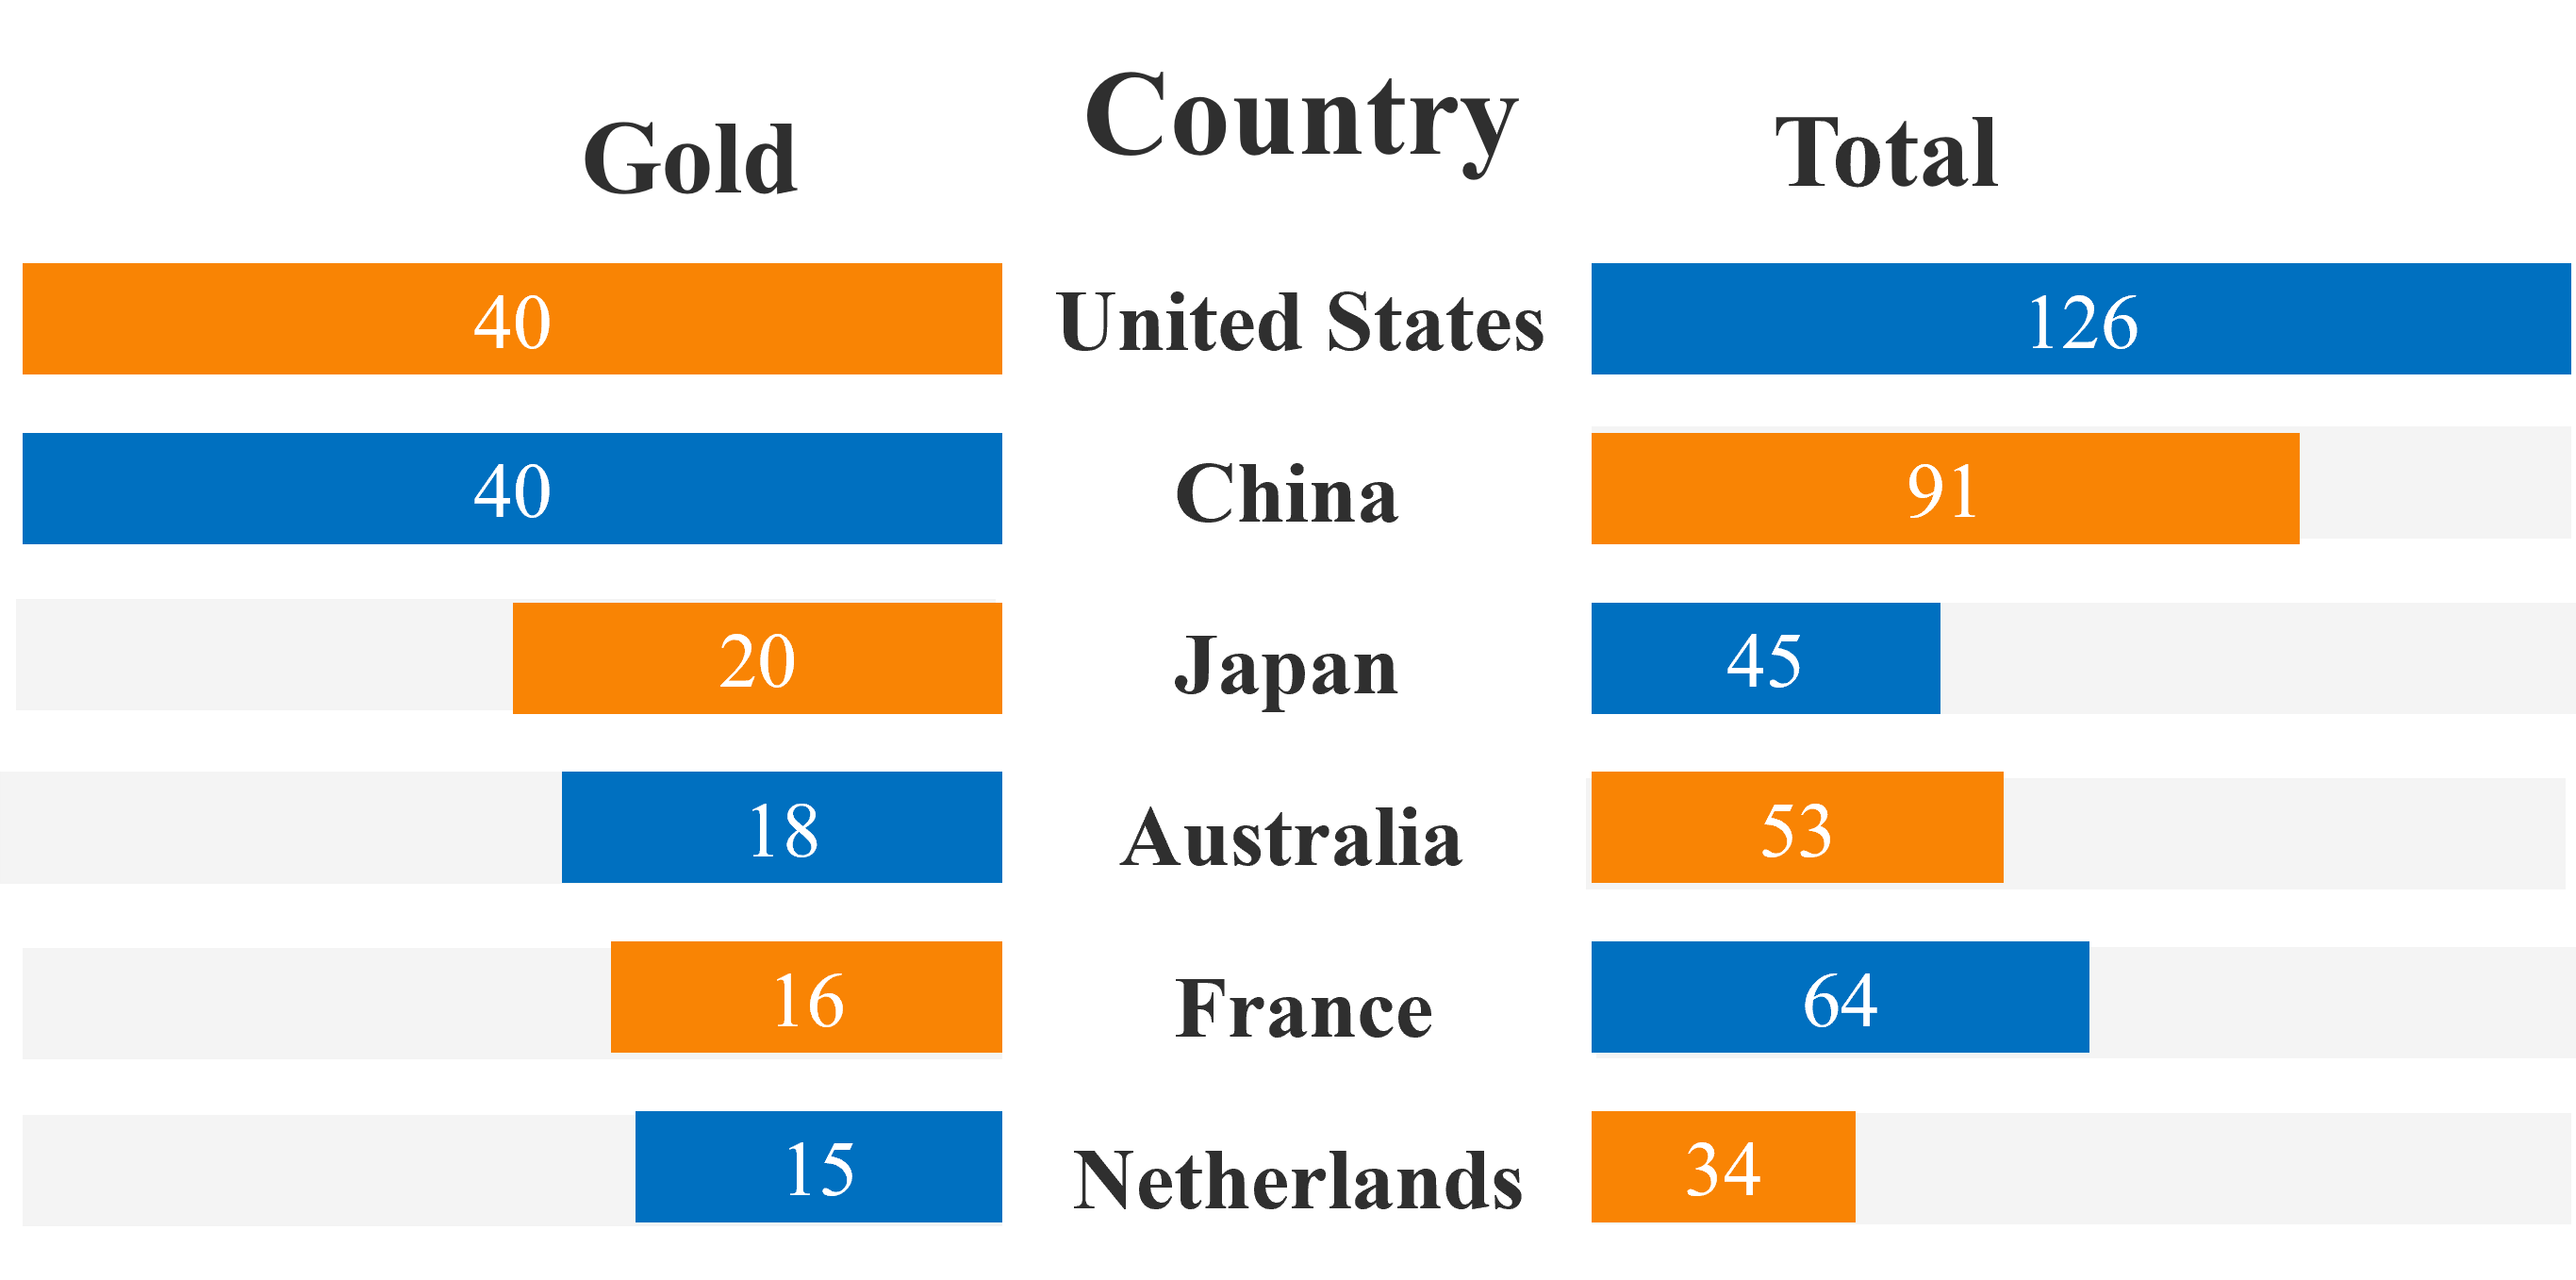
\includegraphics[width=0.8\linewidth]{Paris Olympics(2024) Medal Table - Gold Medals Top 6 Countries.png}
\caption{Paris Olympics(2024) Medal Table - Gold Medals Top 6 Countries}
\end{figure}

\subsection{Restatement of the Problem}
Considering the background information and the results in this file, we need to solve the following problems:

$\star$ Develop a model to predict the number of medals that each country will win at the 2028 Los Angeles Olympics and provide prediction intervals. Predict how many countries may win medals for the first time in 2028, along with probability estimates.

$\star$ Explore the relationship between the setting of Olympic events and the medal-winning situations of various countries.Identify which sports contribute the most to the medal counts of different countries and explain the reasons.

$\star$ Identify the impact of "great coach" on the number of medals through data analysis.Select three countries and analyze which sports they require the introduction of  "great coach", and estimate the potential impact.

$\star$ Provide other original insights revealed by the model regarding the Olympic medal table.
Explain how these insights can provide decision support for country Olympic Committees.

\subsection{Our Work}
The rest of this article is organized as follows. In the second section, we introduced the underlying assumptions and reasons, and in the third section, we mentioned common variables in the formula. In the fourth section, data preprocessing was performed before modeling. The fifth section established a prediction model for the number of medals and provided a prediction interval, exploring the importance of selecting sports events in different countries. The seventh and eighth sections continue to explore the interesting features of data files. In Sections 9 and 10, we analyzed the sensitivity of the model and further evaluated its strengths and weaknesses. Finally, based on our findings, a conclusion was drawn.

\begin{figure}[h] 
\centering
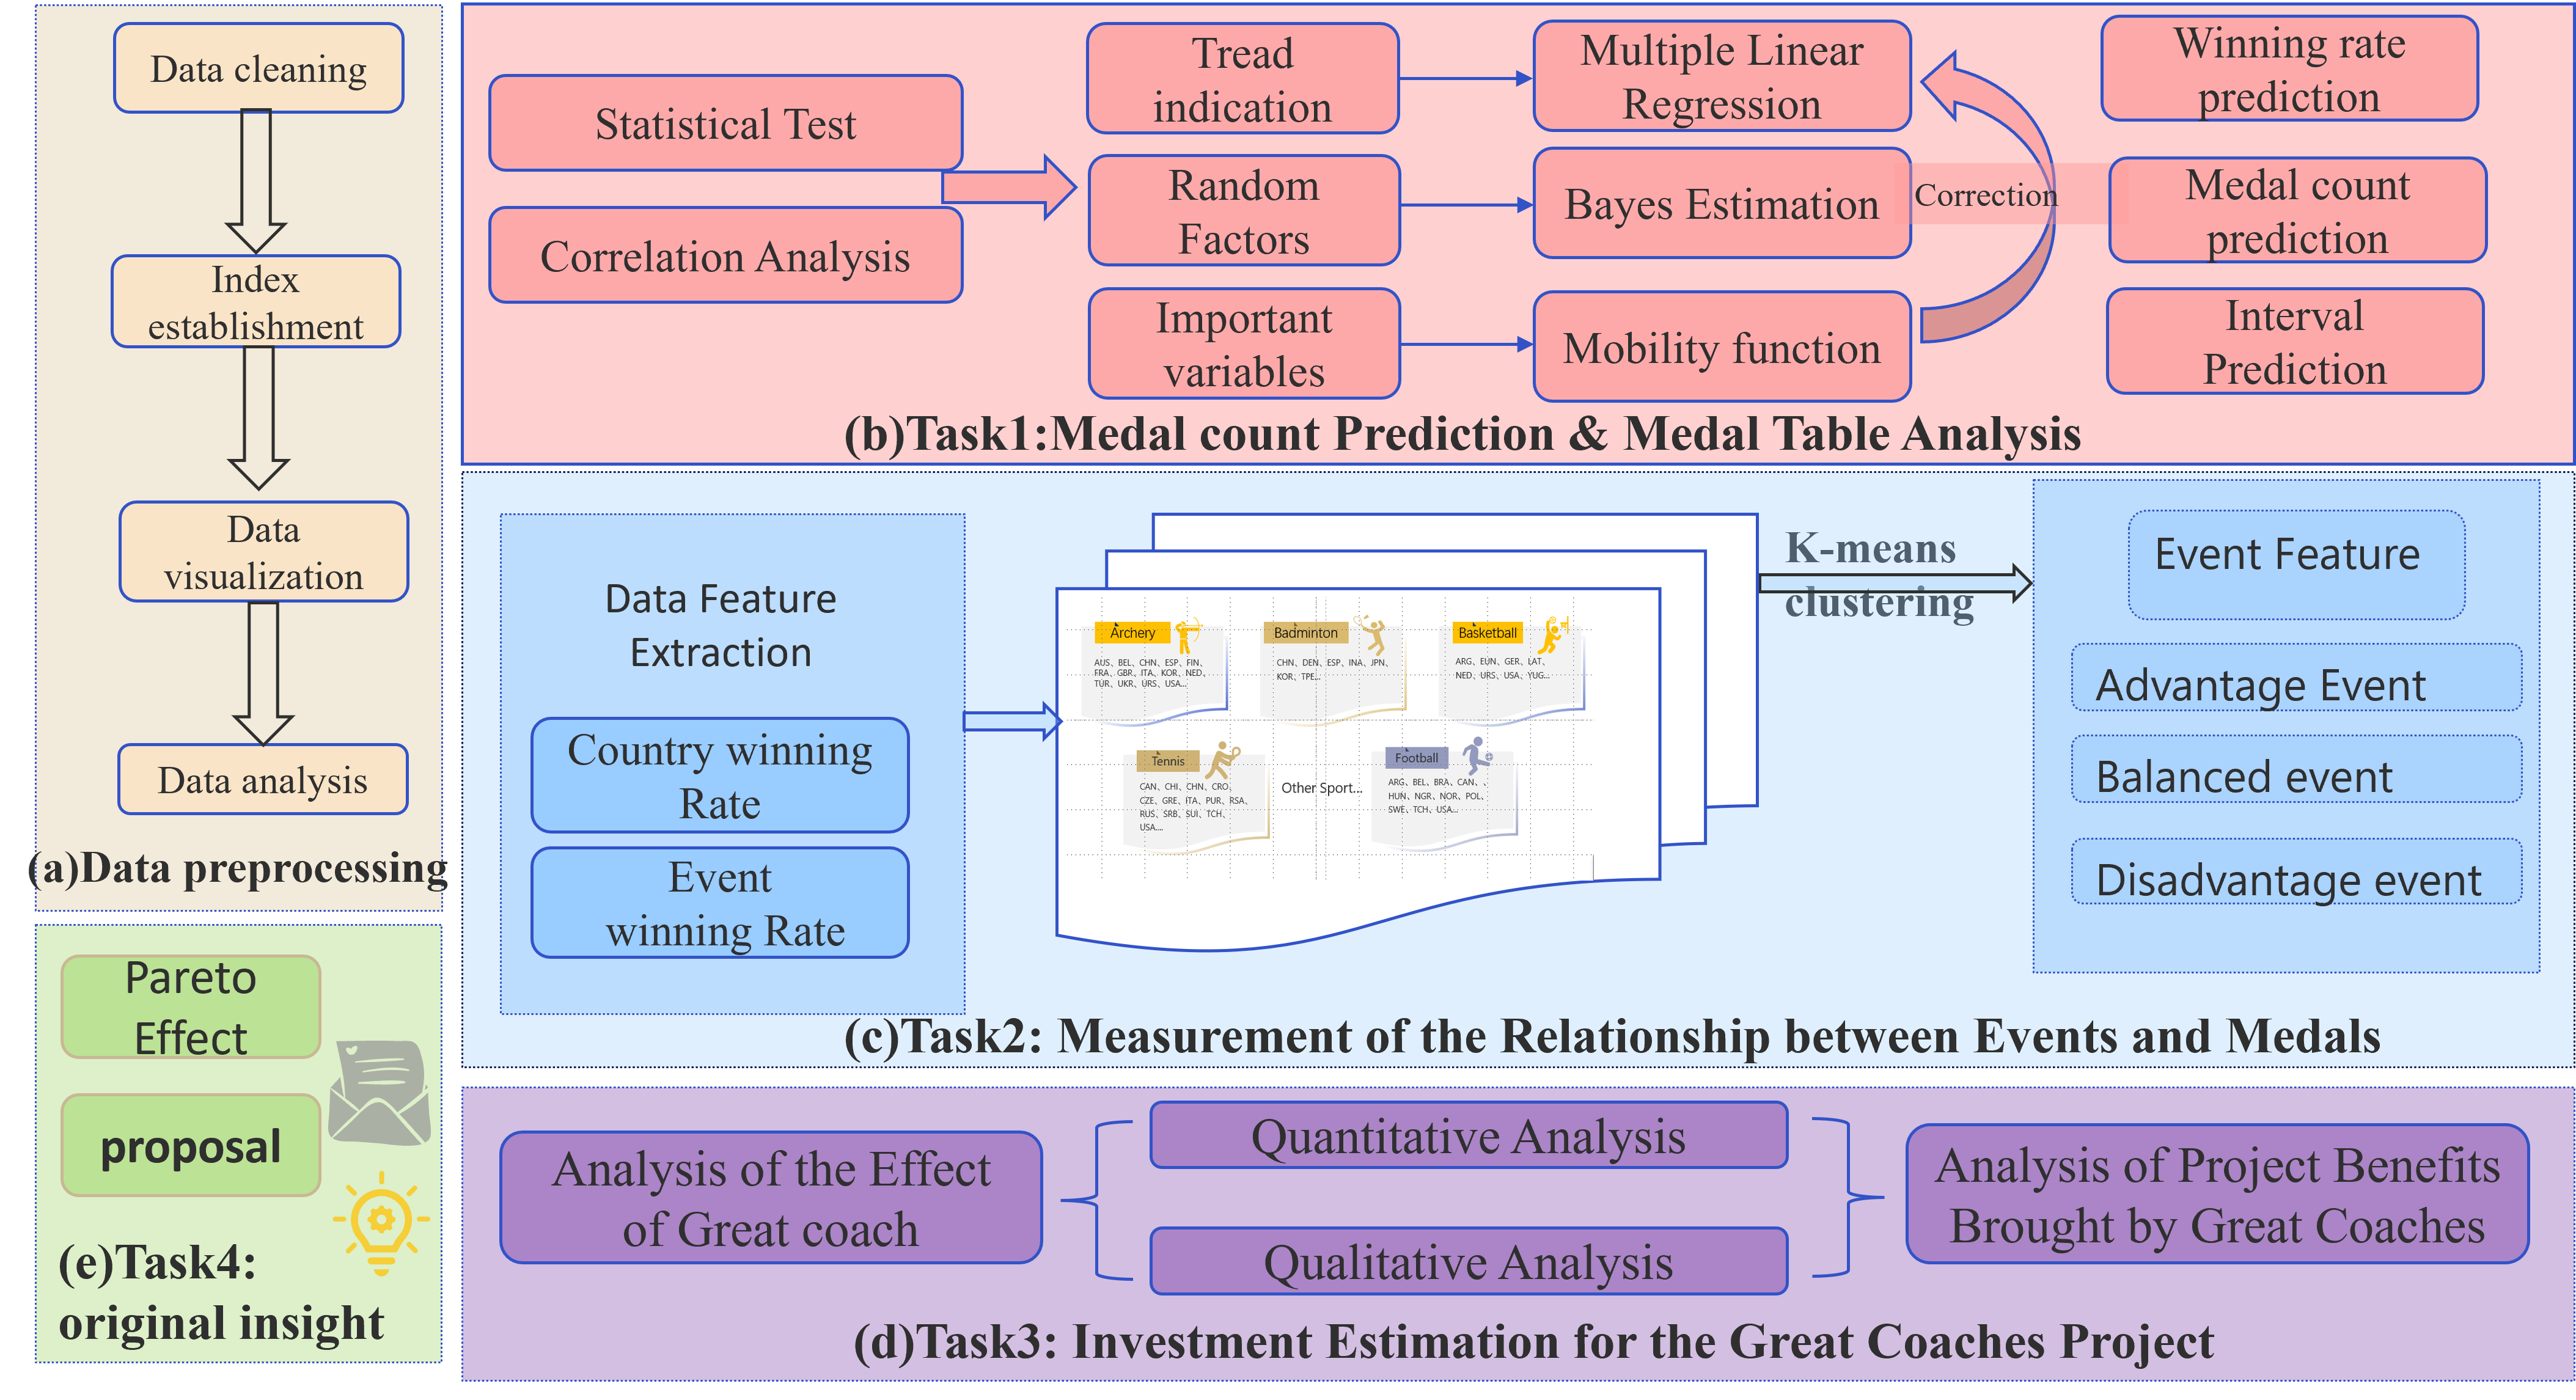
\includegraphics[width=0.8\linewidth]{Our Work.png}
\caption{Our Work}
\end{figure}

\section{Assumptions and Justification}

To simplify the problem and make it convenient for us to simulate real-life conditions, we make the following basic assumptions, each of which is properly justified.

$  \blacklozenge $  {\bf Assumption 1: The countries participating in the 2024 Olympics will continue to participate in the 2028 Olympics.}

{\bf Justification:} Taking into account the core position of the Olympics in international sports exchange, the long-established tradition of participation by various countries, and the multifaceted benefits brought about by participation in the Olympics, including political, economic, and cultural aspects, it is reasonable to assume that the countries participating in the 2024 Olympics will still choose to participate in the 2028 Summer Olympics in Los Angeles, USA.

$  \blacklozenge $  {\bf Assumption 2: The medal performance of each country in different events is independent, meaning that the medal performance of a country in one event does not affect its performance in other events.}

{\bf Justification:} The events in different competitions have varying project settings, participants, and competition rules. Therefore, a country's performance in one event will not directly affect its performance in other events. Thus, it is reasonable to assume that a country's medal performance in one event will not influence its performance in other events.

$  \blacklozenge $  {\bf Assumption 3: Ignoring the influence of athletes' subjective factors, athletes participating in the Olympics are unlikely to withdraw from the competition midway due to a lack of subjective willingness to continue.}

{\bf Justification:} Due to undergoing multiple rounds of selection and long-term training, they are filled with a sense of mission and honor, and the event support and incentives are in place. This assumption can simplify the analysis of competition results and athlete performance, allowing for a focused exploration of the impact of objective factors.

\section{Notations}

\begin{table}[H]
\centering
\begin{tabular}{ll} 
\hline
\textbf{Symbols~ ~ ~ ~ ~ ~~} & \textbf{Description}                                                                                                                                                                                                                                                                                                                  \\ 
\hline
\vcell{$MP^{i}(t)$}                  & \vcell{\begin{tabular}[b]{@{}l@{}}\textcolor[rgb]{0.031,0.031,0.031}{The proportion of the total number of medals won by }\\\textcolor[rgb]{0.031,0.031,0.031}{the i-th country at the t-th Olympic Games.}\\\textcolor[rgb]{0.031,0.031,0.031}{}\end{tabular}}                                                                       \\[-\rowheight]
\printcelltop                & \printcellmiddle                                                                                                                                                                                                                                                                                                                      \\
\vcell{$S\_Num^{i}(t)$}                  & \vcell{\begin{tabular}[b]{@{}l@{}}\textcolor[rgb]{0.031,0.031,0.031}{The total number of events participated by the i-th~}\\\textcolor[rgb]{0.031,0.031,0.031}{country in the t-th Olympic Games.}\\\textcolor[rgb]{0.031,0.031,0.031}{}\end{tabular}}                                                                                \\[-\rowheight]
\printcelltop                & \printcellmiddle                                                                                                                                                                                                                                                                                                                      \\
\vcell{$P\_Num^{i}(t)$}                  & \vcell{\begin{tabular}[b]{@{}l@{}}\textcolor[rgb]{0.031,0.031,0.031}{The number of awards won by athletes from the i-th }\\\textcolor[rgb]{0.031,0.031,0.031}{country in the t-th Olympic Games.}\\\textcolor[rgb]{0.031,0.031,0.031}{}\end{tabular}}                                                                                 \\[-\rowheight]
\printcelltop                & \printcellmiddle                                                                                                                                                                                                                                                                                                                      \\
\vcell{$M_{i, j}(t)$}                  & \vcell{\begin{tabular}[b]{@{}l@{}}\textcolor[rgb]{0.031,0.031,0.031}{The number of awards won by country i in event j at }\\\textcolor[rgb]{0.031,0.031,0.031}{the t-th Olympic Games.}\\\textcolor[rgb]{0.031,0.031,0.031}{}\end{tabular}}                                                                                           \\[-\rowheight]
\printcelltop                & \printcellmiddle                                                                                                                                                                                                                                                                                                                      \\
\vcell{$S_{i, j}(t)$}                   & \vcell{\begin{tabular}[b]{@{}l@{}}\textcolor[rgb]{0.031,0.031,0.031}{The total number of athletes from country i }\\\textcolor[rgb]{0.031,0.031,0.031}{participating in event j at the t-th Olympic Games.}\\\textcolor[rgb]{0.031,0.031,0.031}{}\end{tabular}}                                                                       \\[-\rowheight]
\printcelltop                & \printcellmiddle                                                                                                                                                                                                                                                                                                                      \\
\vcell{$\hat{MP_{j}^{i}}$}                   & \vcell{\begin{tabular}[b]{@{}l@{}}\textcolor[rgb]{0.031,0.031,0.031}{The j-th predicted value for country i obtained through }\\\textcolor[rgb]{0.031,0.031,0.031}{a multiple linear regression model based on the }\\\textcolor[rgb]{0.031,0.031,0.031}{independent variables.}\\\textcolor[rgb]{0.031,0.031,0.031}{}\end{tabular}}  \\[-\rowheight]
\printcelltop                & \printcellmiddle                                                                                                                                                                                                                                                                                                                      \\
\vcell{$X^{i}(t)$, $Y^{i}(t)$, $Z^{i}(t)$}                  & \vcell{\begin{tabular}[b]{@{}l@{}}\textcolor[rgb]{0.031,0.031,0.031}{The number of gold, silver, and bronze medals won by }\\\textcolor[rgb]{0.031,0.031,0.031}{country i in year t.}\\\textcolor[rgb]{0.031,0.031,0.031}{}\end{tabular}}                                                                                             \\[-\rowheight]
\printcelltop                & \printcellmiddle                                                                                                                                                                                                                                                                                                                      \\
\vcell{$Item_{i, j}(t)$}                   & \vcell{\textcolor[rgb]{0.031,0.031,0.031}{The index of advantage for country i in event j in year t.}}                                                                                                                                                                                                                                \\[-\rowheight]
\printcelltop                & \printcellmiddle                                                                                                                                                                                                                                                                                                                      \\
\hline
\end{tabular}
\end{table}

where we define the main parameters while specific value of those parameters will be given later.

\section{Data Pre-processing}
\subsection{Data Overview}
Conduct a general analysis of the data as shown in Figure 3.

\begin{figure}[h] 
\centering
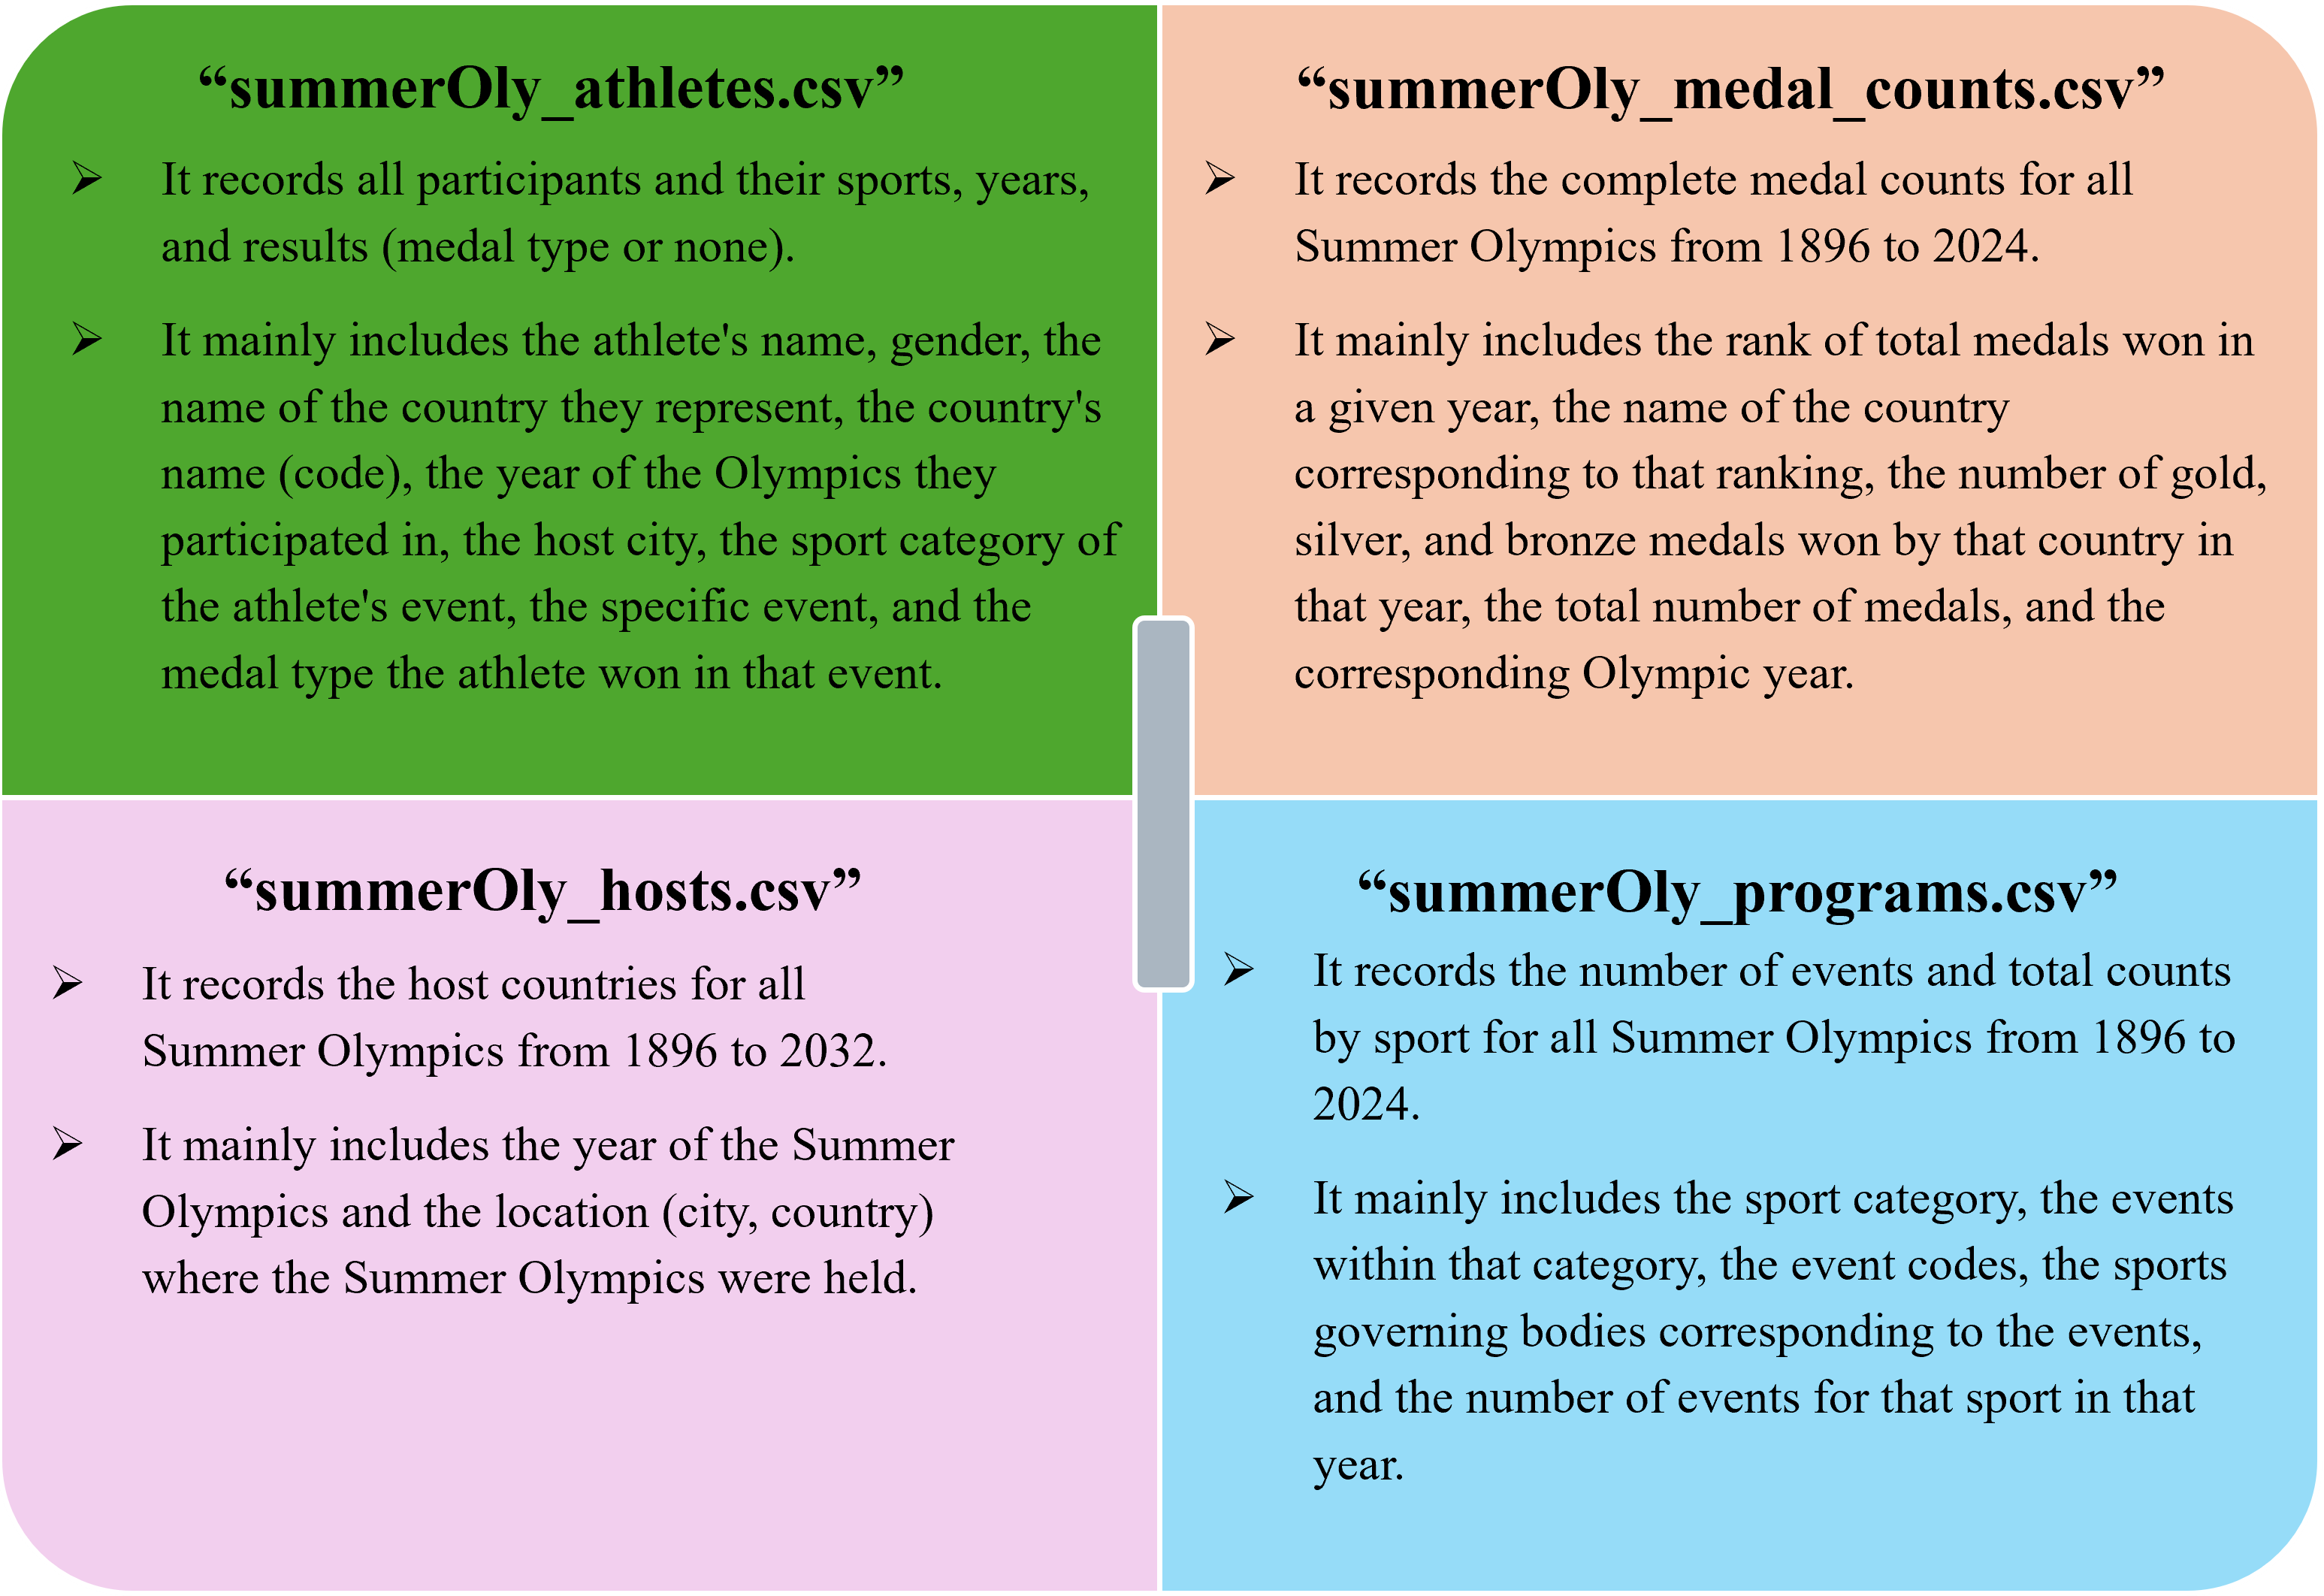
\includegraphics[width=10cm]{Overview of four data tables.png}
\caption{Overview of four data tables} \label{fig1}
\end{figure}

Notably: 

a) In 1936, during Nazi Germany, the Berlin Olympics was boycotted.

b) In 1980, during the Cold War, the Moscow Olympics was boycotted by the West. 

c) In 1984, during the Cold War, the Soviet Union boycotted the Los Angeles Olympics in the United States. 

These significant historical events caused large fluctuations in medal counts, resulting in some countries having zero medals, which can be analyzed further.

Encoding detection of the provided dataset files is shown in Table 1.

\begin{table}[h]
\centering
\caption{Data files and encoding formats}
\begin{tabular}{|l|l|} 
\hline
File                                  & Encoding                 \\ 
\hline
\textbf{data\_dictionary.csv}         & \textbf{windows 1252}    \\ 
\hline
\textbf{summerOly\_athletes.csv}      & \textbf{UTF-8}           \\ 
\hline
\textbf{summerOly\_hosts.csv}         & \textbf{UTF-8 with BOM}  \\ 
\hline
\textbf{summerOly\_medal\_counts.csv} & \textbf{UTF-8}           \\ 
\hline
\textbf{summerOly\_programs.csv}      & \textbf{windows 1252}    \\
\hline
\end{tabular}
\end{table}

For convenience in subsequent processing, the above files were uniformly converted to .xlsx files in UTF-8 encoding format.

\subsection{Data Cleaning}
\subsubsection{In "summerOly_athletes.csv" file}
\hskip\parindent a) There is an athlete named "671" in row 244172, which is clearly not a valid name. To facilitate subsequent unified processing, after checking other information about the athlete, the name was corrected to Liu Qinglian.

b)Duplicate value check revealed 1466 duplicate rows in the file, which have been deduplicated.

c)The presence of an outlier of 0 in the total medal count for all countries in the following sports indicates that no country won any medals in those sports that year, which is clearly unreasonable. Therefore, these categories of sports should be removed.

\begin{figure}[h] 
\centering
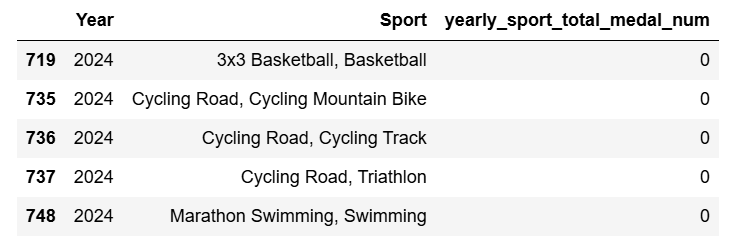
\includegraphics[width=0.8\linewidth]{The statistical situation of the abnormal Sport category.png}
\caption{The statistical situation of the abnormal Sport category} \label{fig1}
\end{figure}

\subsubsection{In "summerOly_programs.csv" file}
\hskip\parindent a) There are encoding issues, suspected to be due to encoding problems, so it was processed using the Windows 1252 encoding. 

b) There are missing values in the programs.csv file. The detailed missing situation is shown in Figure 2.

\begin{figure}[h] 
\centering
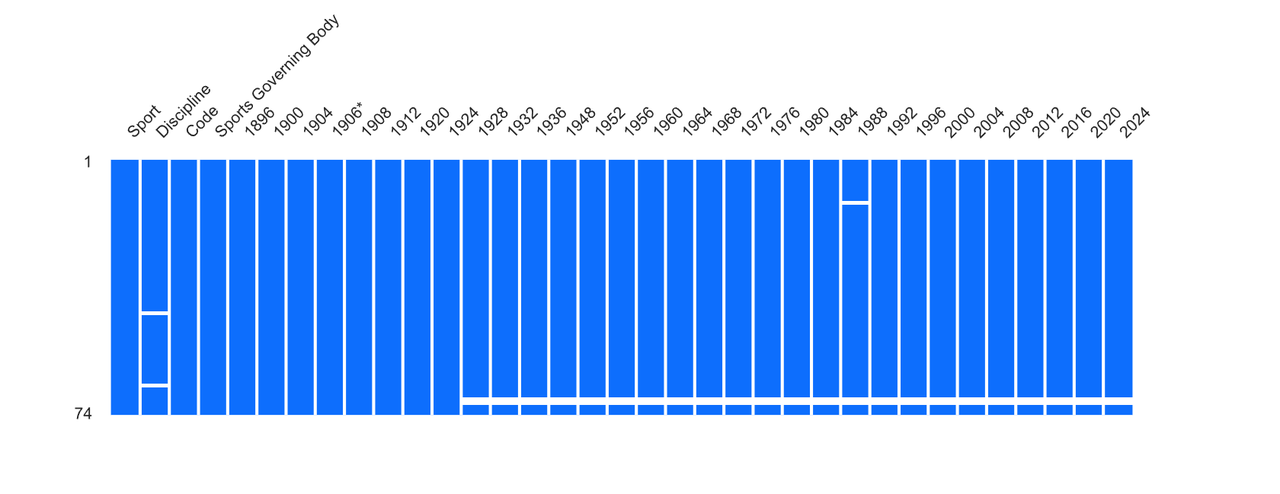
\includegraphics[width=10cm]{Schematic diagram of missing values in the programs table.PNG}
\caption{Schematic diagram of missing values in the programs table} \label{fig1}
\end{figure}
i.The value for 1988 in row 14 is missing.

ii.Figure skating and ice hockey, which are ice sports, were held at the Summer Olympics before 1924. However, they were moved to the first Winter Olympics in 1924, so the values for figure skating and ice hockey in rows 71 and 72 for 1924 and later are missing. 

iii.Because Modern Pentathlon and Water Motorsports do not have further classifications, the “Discipline” values are missing in rows 46 and 67. Based on other data analysis, the “Sport” values of the row was filled into the “Discipline” values. 

\subsubsection{In "summerOly_athletes.csv" and "summerOly_hosts.csv" files}
\hskip\parindent a)Datas for the year {1906} exist in “summerOly_athletes.csv” file but not in the hosts.csv file.

$\bigtriangleup$ Reason: According to research, an unofficial Olympics was held in Athens, Greece, in 1906. 

b)Datas for the years {2028, 2032, 1944, 1940, 1916} exist in “summerOly_hosts.csv” file but not in “summerOly_athletes.csv” file. 

$\bigtriangleup$ Reason: The Olympics for the years {2028, 2032} have not yet taken place. The host countries and cities have been determined, but the participating athletes have not been determined. The three Olympics originally scheduled for the years {1944, 1940, 1916} were canceled due to the two world wars in the 20th century. Although the hosts had been determined, there was no list of participating athletes because they could not be held.

\subsubsection{In "summerOly_medal_counts.csv" file}
\hskip\parindent After reading with UTF-8 encoding, it was found that the 'NOC' column had trailing spaces. All strings in this column were processed to remove excess leading and trailing spaces.

\section{Task 1}

\subsection{ Analysis of the Factors Influencing National Olympic Medal Counts from a Multidimensional Perspective}
The number of Olympic medals won by a country reflects its overall strength and is influenced by multiple factors. Based on the existing dataset, we extract feature information to identify the important factors that affect the number of Olympic medals won by various countries. We then select significant features to analyze the quantity of Olympic medals.

It can be observed that the total number of medals won by each country is related to many factors, with the most significant influencing factors being the total number of events participated in by the country in the Olympics, the medal results of its athletes, the total number of medals won by the country in previous Olympic Games, and whether the country is the host nation.

(1) Total number of events participated in by the country in the Olympics: Analysis of the data reveals a significant positive correlation between the number of events participated in and the total number of medals. The more events participated in, the greater the competitive capacity of the country across various fields, thus increasing the chances of winning medals.

(2) Number of medals won by athletes: This article quantifies the competitive level of athletes based on their medal results in the events participated in. The more medals won by an athlete, the higher their competitive level is indicated to be. In the aforementioned correlation analysis, there is a significant correlation between the total number of medals won by the countries and this factor.

(3) Total number of medals won by the country in previous Olympic Games: Analyzing the medal data from past Olympic Games shows that the total number of medals has a certain degree of continuity and stability. Correlation analysis also indicates a significant correlation with this factor.

(4) Host nation effect: The host nation effect is a phenomenon widely studied and highly regarded in the competitive landscape of the Olympics. The correlation analysis above indicates that it has some influence on the number of medals won by the host country. Further examination through the Wilcoxon signed-rank test of the host advantage reveals that there is a significant difference between the number of medals won by the host nation and its previous medal count, further validating the impact of the host nation effect on the medal counts of countries.

\subsection{Sub-model I:A Multivariate Linear Regression-Based Model for Predicting the Total Medal Count of Countries in the Olympics}

\subsubsection{Model Preparation}
\hskip\parindent From the systematic analysis of influencing factors in the earlier stages, we know that the competitive performance of various countries in the Olympics, specifically quantified as the proportion of the total number of medals won in Olympic competitions, is closely related to the proportion of the total number of events in which the country participates in that year's Olympics. At the same time, the past performance of the country in the Olympics, especially in the previous year and recent years, has a significant and undeniable impact on the total number of medals for the current session.

Based on these factors, let $MP^{i}(t)$ represent the proportion of total medals won by the $i$-th country in the $t$-th Olympics; $S\!-\!Num^{i}(t)$ represents the total number of events participated in by the $i$-th country in the $t$-th Olympics; $P\!-\!Num^{i}(t)$ is the number of medals awarded to athletes from the $i$-th country in the $t$-th Olympic Games; $Home^{i}(t)$is a dummy variable, when the $i$-th country is the host country of the $t$-th Olympics, $Home^{i}(t)=1$, otherwise it equals 0.

\subsubsection{Model Establishment}
\hskip\parindent Because $MP^{i}(t)$ represents the medal-winning rate of each country, it takes values between 0 and 1. We perform a logarithmic transformation on $S\_Num^{i}(t)$ and $P\_Num^{i}(t)$, namely: $S\_Num^{i}(t) = log(S\!-\!Num^{i}(t) + 1)$, $P\_Num^{i}(t) = log(P\!-\!Num^{i}(t) + 1)$.
Thus, it satisfies
\begin{align} \label{eq1}
\notag
MP^{i}(t, \theta) = a_{1}^{i} + a_{2}^{i} \times S\_Num^{i}(t) + a_{3}^{i} \times P\_Num^i(t) \\ 
+ a_{4}^{i} \times Home^{i}(t) + a_{5}^{i} \times MP^{i}(t - 4) + \varepsilon^{i}(t)
\end{align}

Where, $\theta = [a_{1}, a_{2}, a_{3}, a_{4}, a_{5}]$ is the regression coefficient; $t$ is the year of hosting the Olympics; $\varepsilon ^{i}(t)$ encompasses all uncertain factors.

Then we fit it using the least squares method. Let $y^{i}(t)$ be the observed value for the $i$-th country in the $t$-year Olympics. The regression result is $\hat{MP}^{i}(t, \hat{\theta })=\sum_{j=1}^{5}a_{j}^{i}\times f^{i}(t, j)$, and the loss function is $L(\hat{\theta }) = \sum_{t}[y^{i}(t)-\hat{M}^{i}(t, \hat{\theta})]^2$. The parameter estimate that minimizes 
$\hat{\theta }$ is taken as $L(\hat{\theta })$, thus $\hat{MP}^{i}(t, \hat{\theta })$ is the regression outcome.

The total number of medals at each Olympic Games is not constant; it is determined by a combination of factors such as the events contested and the athletes' conditions. The changes in the total number of medals at each Olympic Games over time are illustrated in FigureXXX:

\begin{figure}[H] 
\centering
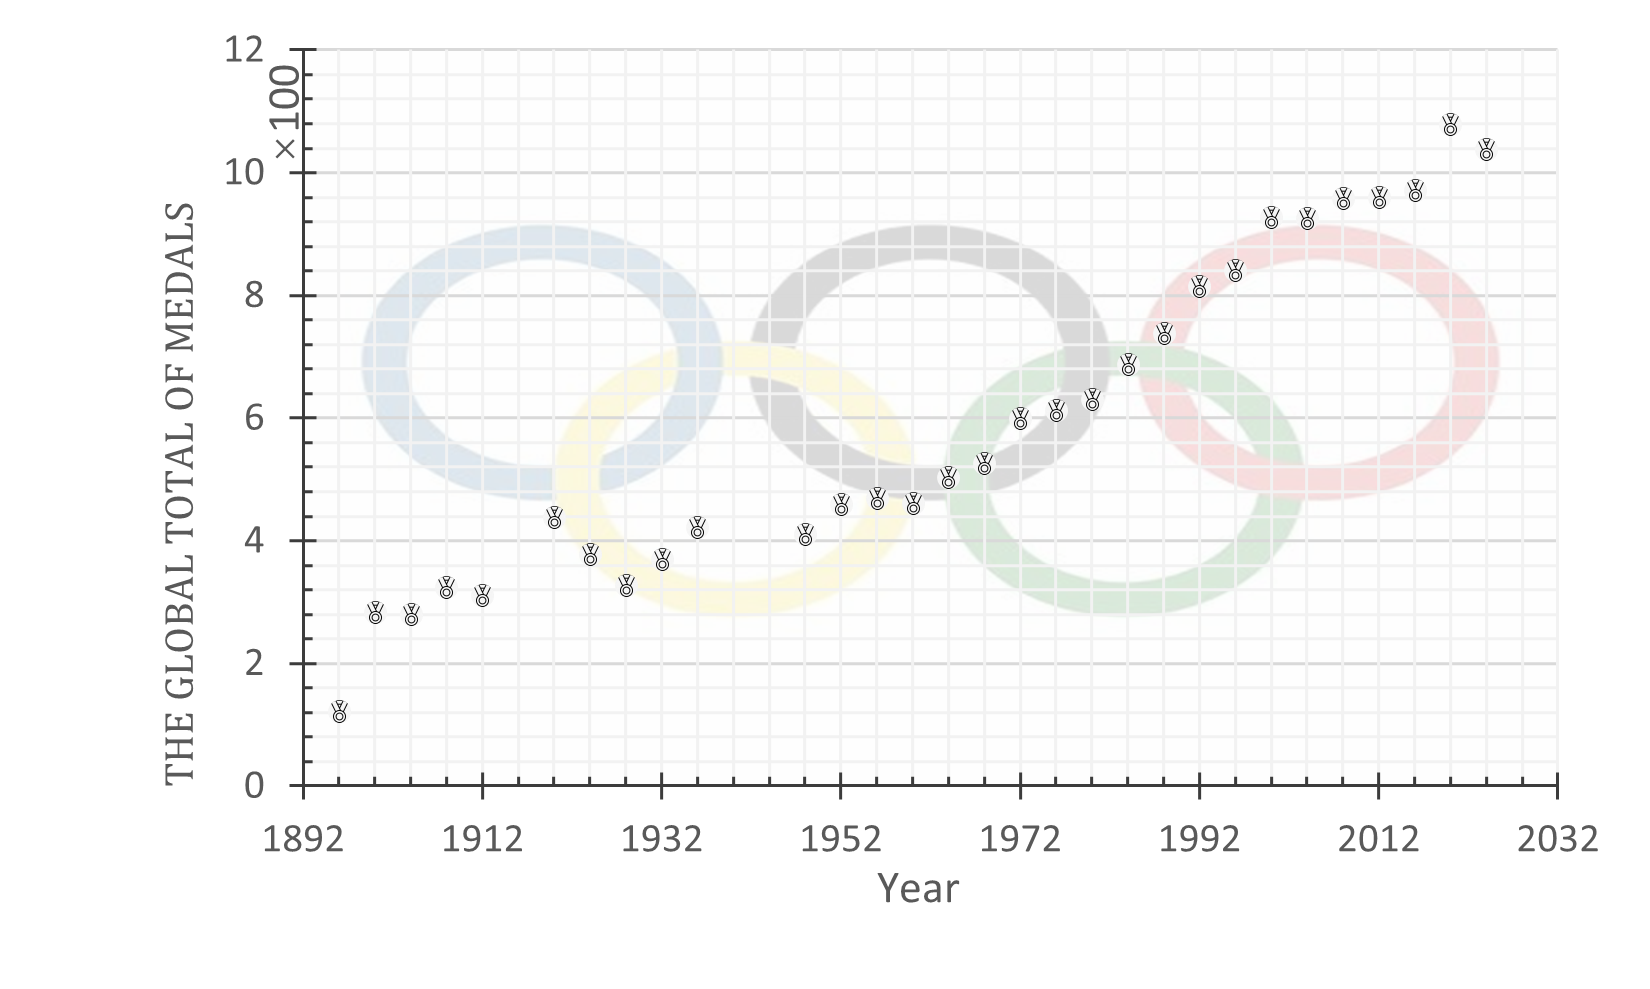
\includegraphics[width=10cm]{Global Total Olympic Medals Over Time.png}
\caption{Global Total Olympic Medals Over Time}
\end{figure}

From the analysis of the above figure, it can be seen that the total count of each Olympic Games shows a linear trend over time. It is noted that data points for the years 1916, 1940, and 1944 are missing, as during these years the Olympics were cancelled due to historical events, thus no records exist. The scatter plot above indicates a generally linear trend. Therefore, we employ a linear function to fit this trend.
\begin{equation}
M\_Sum = \beta_{0} + \beta_{1}t
\end{equation}

Where, $\hat{\beta} = [\beta_{0}, \beta_{1}]$ is the regression coefficient; $t$ refers to the year of the Olympics $-1892$.

We employ OLSE to estimate $\hat{\beta}$, and predict that the total number of medals for the years 2028 and 2032 in Table XXX.

\begin{table}[h]
\centering
\caption{The prediction of the total number of medals.}
\begin{tabular}{|c|c|c|} 
\hline
Year     & ~ 2028~~ & ~ 2032~~  \\ 
\hline
Pre\_Sum & 1026     & 1052      \\
\hline
\end{tabular}
\end{table}
Combining the medal-winning rates of various countries with the predictions of the total number of Olympic medals, $ Me^{i}(t) = Sum\_M(t)\times MP^{i}(t)$, based on $Me^{i}(t)$, we can predict the standings on the medal table.

\subsection{Sub-model II: Exploring the Medal Distribution of Countries Based on Bayesian Models}
\subsubsection{Model Preparation}
\hskip\parindent In the above model construction, we can predict the total medal counts for each country. Let the total number of medals be $N$, with $X$, $Y$, and $Z$ representing the number of gold, silver, and bronze medals respectively, then $N=X+Y+Z$.

If we rank by scoring system, then the total score is $S=W_{1}\times X+W_{2}\times Y+W_{3}\times Z$, with countries scoring higher ranking ahead; if ranked by total medal count, then $S=N$, with countries winning more medals ranking higher.

Based on historical data and experience regarding countries' medal counts, we know that athletes participating in the Olympics can fall into one of four categories: gold medalists, silver medalists, bronze medalists, and those who unfortunately do not win any medals. At the early stages of the competition, we cannot ascertain the true capabilities of participating athletes, thus we can only predict that the probabilities of these four outcomes for each athlete are equal. Similarly, within the total medals awarded to each country, we use a multinomial distribution as the prior distribution, that is 

\begin{equation}
(X, Y, Z|N)\sim Multinomial(N, p_{1}, p_{2}, p_{3})
\end{equation}
 
Where, $p_{1}$, $p_{2}$, and $p_{3}$ are the prior probabilities of gold, silver, and bronze medals, respectively; and $p_{1}+p_{2}+p_{3}=1$.

\subsubsection{Model Establishment}
\hskip\parindent Based on the specific medal counts of various countries, $D^i(t)={X^{i}(t), Y^{i}(t), Z^{i}(t)}$ represents the number of gold, silver, and bronze medals country $i$ wins in $t$ year.

Here, $i\in \{France, United States, Germany, Australia, ...\}$, $t\in \{1896, 1900, ...,2024\}$.

Assuming the observations for year $t$ from country $i$ are independent and identically distributed given the winning situation, the sample likelihood function can be expressed as $P(D^{i}|X^{i}, Y^{i}, Z^{i})= \prod_{t}(p(x^{i}(t), y^{i}(t), z^{i}(t)|X, Y, Z)$.

Under the assumption of a multinomial prior distribution, for every group of historical sample data, $(x^{i}(t), y^{i}(t), z^{i}(t))$, its probability distribution can be expressed as $P(x^{i}(t), y^{i}(t), z^{i}(t)|N)=\frac{N!}{x^{i}!y^{i}!z^{i}!}P_{1} ^{x^{i}}P_{2} ^ {y^{i}}P_{3} ^ {z^{i}}$, thus the likelihood function is $P(D|X, Y, Z)=\prod_{i=1}^{n}\frac{N!}{x^{i}!y^{i}!z^{i}!}P_{1}^{x^{i}}P_{2}^{y^{i}}P_{3}^{z^{i}}$.

Substituting the prior distribution and the likelihood function into the equation, and computing the normalization constant C ensures that $\sum_{x+y+z=N}P(X=x, Y=y, Z=z|D)=1$.

Thus, the posterior distribution can be expressed as: $P(X^{i}(t), Y^{i}(t), Z^{i}(t)|D) = \frac{1}{c} \times \frac{N!}{x!y!z!}P_{1}^{x}P_{2}^{y}P_{3}^{z}\prod_{t=1}^{n}\frac{N!}{x^{i}(t)!y^{i}(t)!z^{i}(t)!}P_{1}^{x^{i}(t)}P_{2}^{y^{i}(t)}P_{3}^{z^{i}(t)}$.

By introducing the Bayesian model, in combination with the prior distribution and historical data, we can effectively evaluate the number of gold medals won given the total number of medals is known.

\subsection{Model Improvement Based on Advantage Project Relaxation Function}
As the medal count does not adequately measure the ability of athletes from countries that have never won any medals, we modify the multiple linear regression model. In this case, the assessment of athletes' capabilities from a country is not only based on the total count of medals won but also considers all data regarding the events and awards of athletes provided in the data set, including results from unofficial competitions. Thus, we adjust the independent variable $P\_Num^{i}(t)$ to ensure $P_{1}\_Num^{i}(t) = P+P\_Num^{i}(t)$, where $P$ indicates the minimum level of the country's athletes, measured by the participation rate in events from that country. Additionally, the effect of project advantages also influences the medal-winning outcomes of countries to some extent. By considering the number and types of events, we adjust the independent variable $S\_Num^{i}(t)$ as follows:
\begin{equation}
S_{1}\_Num^{i}(t) = S\_Num^{i}(t) + f(p)
\end{equation}

Where, $f(p) = \sum_{k=1}^{n}w_{k}I_{k}$ and $w_{k}$ represent the weight proportions for various projects; $I_{k}$ represents the count variable for project types.

Therefore, the modified multiple linear regression function is $MP^{i}(t, \theta) = a_{1}^{i}+a_{2}^{i}\times S_{1}\_Num^{i}(t) + a_{3}^{i}\times P_{1}\_Num^{i}(t) + a_{4}^{i}\times H^{i}(t) + a_{5}^{i}MP^{i}(t-4)$.

Since the previously mentioned random variables $X^{i}(t)$, $Y^{i}(t)$, and $Z^{i}(t)$ do not constitute a completely independent variation process in practice, their random fluctuations and magnitudes are influenced by the types and number of events that the country participates in, thus the values of $P_{1}^{i}(t)$, $P_{2}^{i}(t)$, and $P_{3}^{i}(t)$ will change with the number and type of events, as categorized below:

\begin{equation}
Item_{i, j}(t) = \frac{M_{i, j}(t)}{S_{i, j}(t)} \times \frac{P\_Num^{i}(t)}{S\_Num^{i}(t)}
\end{equation}

Where, $M_{i, j}(t)$ represents the number of medals won by country $i$ in event $j$ at the Olympic Games in year $t$; $S_{i, j}(t)$ represents the total number of athletes from country $i$ participating in event $j$ at the Olympic Games in year $t$. The indicators can be defined as follows:
(1)Advantage Projects: The country has a strong capability in this event, with high athlete skill levels, a comprehensive training system, and a history of good performances in major competitions, resulting in a high probability of winning medals. Specifically, when $Item_{i, j}(t)\in (0.6, 1)$, it indicates that this event has long been a superior event for the country.

(2)Balanced Projects: The country has an average capability in this event, with a gap compared to the top levels, yet possesses certain competitive strengths, offering a possibility of winning but with some instability. Specifically, when it $Item_{i, j}(t)\in [0.4, 0.6]$, it indicates that this event has long been a balanced event for the country.

(3)Disadvantage Projects: The country is lagging in this event, with athletes' levels, training conditions, and competitive experience far behind other countries, making it very difficult to win medals. Specifically, when $Item_{i, j}(t)\in (0, 0.4)$, it indicates that this event has long been an inferior event for the country.

Analyzing the "summerOly_programs.csv" and "summerOly_athletes.csv" datasets reveals that certain countries have clear advantages in specific sports. As shown in the chart below, countries like AUS and BEL demonstrate significant strengths in archery, with their superiority index being above 0.6. This indicates that for these countries, participating in shooting sports would be beneficial to their total medal count.

\begin{figure}[h] 
\centering
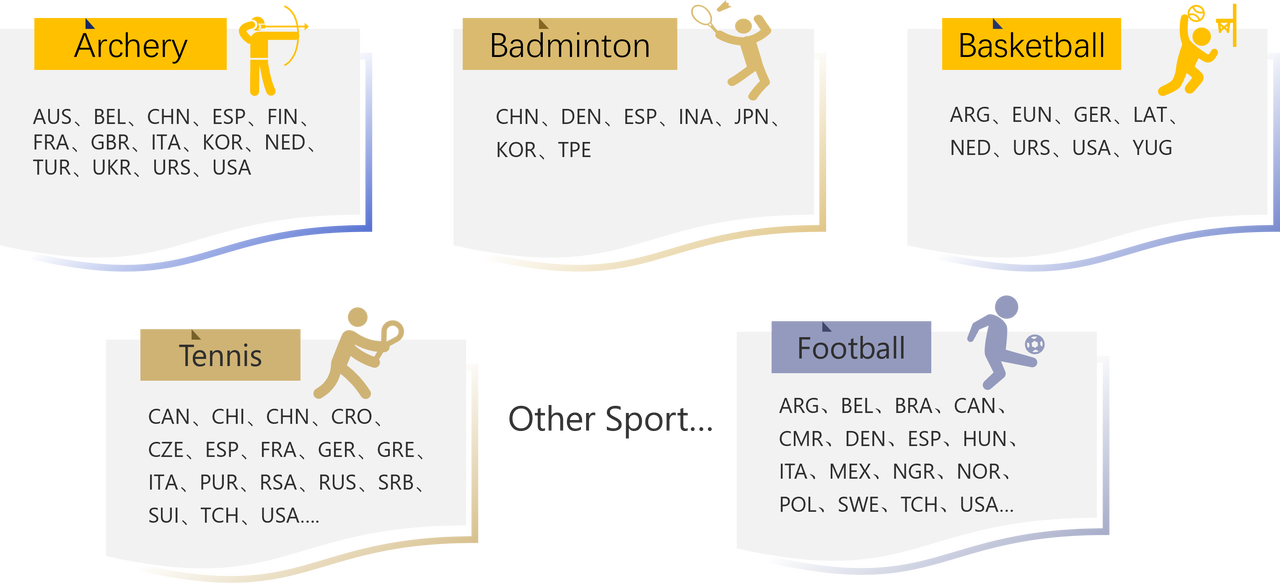
\includegraphics[width=10cm]{Advantageous projects and corresponding countries.png}
\caption{Advantageous projects and corresponding countries}
\end{figure}

We observe that when a project is an advantage project for the country, there is a higher likelihood of winning gold medals, while performance in non-advantage projects is less optimistic. Therefore, we introduce an advantage project relaxation function $f(M)$ to correct the Bayesian model $P_{j}^{oi}(t) = P_{j}^{i}(t)f(M)$.

Therefore, the revised Bayesian estimate replaces $P_{1}$ with $P_{1}^{o}$, and by applying the Newton iterative algorithm, we can obtain the estimated value of $P_{1}^{o}$, thus predicting the number of gold medals each country will win as $Me^{i}\times P_{1}^{oi}$.

\begin{table}
\centering
\caption{ The prediction of the award situations in 2028}
\begin{tabular}{ccc|ccc} 
\hline
\multicolumn{3}{c|}{Top 10}         & \multicolumn{3}{c}{Bottom 10}            \\ 
\hline
Country      & ~ rank~~ & ~ Medal~~ & ~ ~ ~Country~ ~~ & ~ rank~~ & ~ Medal~~  \\ 
\hline
UnitedStates & 1        & 106       & Hungary          & 11       & 23         \\
China        & 2        & 87        & Cuba             & 12       & 22         \\
GreatBritain & 3        & 82        & Canada           & 13       & 20         \\
Germany      & 4        & 59        & Ukraine          & 14       & 19         \\
Australia    & 5        & 47        & Brazil           & 15       & 18         \\
Italy        & 6        & 42        & Spain            & 16       & 18         \\
Japan        & 7        & 42        & Sweden           & 17       & 16         \\
SouthKorea   & 8        & 35        & Kenya            & 18       & 15         \\
Netherlands  & 9        & 27        & Norway           & 19       & 15         \\
France       & 10       & 23        & Poland           & 20       & 15         \\
\hline
\end{tabular}
\end{table}

\subsection{Uncertainty analysis of the influence model}
The dataset we possess and the selected data features may not adequately represent all the factors influencing a country's medal wins, which could lead to some bias in our model. While multiple linear regression categorizes uncertainties as a random error term, the estimation of this random error term also carries bias. The limitations of the data we face when studying the factors affecting a country’s performance in Olympic Games and similar events cannot be overlooked. The current dataset we have has a limited source and cannot comprehensively cover all potential influencing factors. Additionally, the chosen data features are based solely on existing knowledge and analytical frameworks, reflecting only a portion of the factors related to winning medals, making it difficult to fully represent all the factors that influence a country's medal wins.

In multiple linear regression, the residual $e^{i}$ is the difference between the observed value $MP^{i}_{j}$ and the model's predicted value $\hat{MP}^{i}_{j}$, calculated using the following formula:

\begin{equation}
e^{i}_{j} = MP^{i}_{j}-\hat{MP}^{i}_{j}
\end{equation}

Where, $MP_{j}^{i}$ represents the $j$-th observation of country $i$; $\hat{MP}_{j}^{i}$ is the predicted value for country $i$'s $j$-th observation calculated by the multiple linear regression model based on the independent variables.
By conducting multiple linear regression for all participating countries in the Olympic Games and performing statistical analysis on the residuals, we find that the mean residual for each country is 0, with no heteroscedasticity, $E(e^{i}_j) = 0$, and the standard deviation is also within an acceptable range.
The regression results for some countries are shown in the chart below:

\begin{figure}[htbp]
	\centering
	\begin{minipage}{0.4\linewidth}
		\centering
		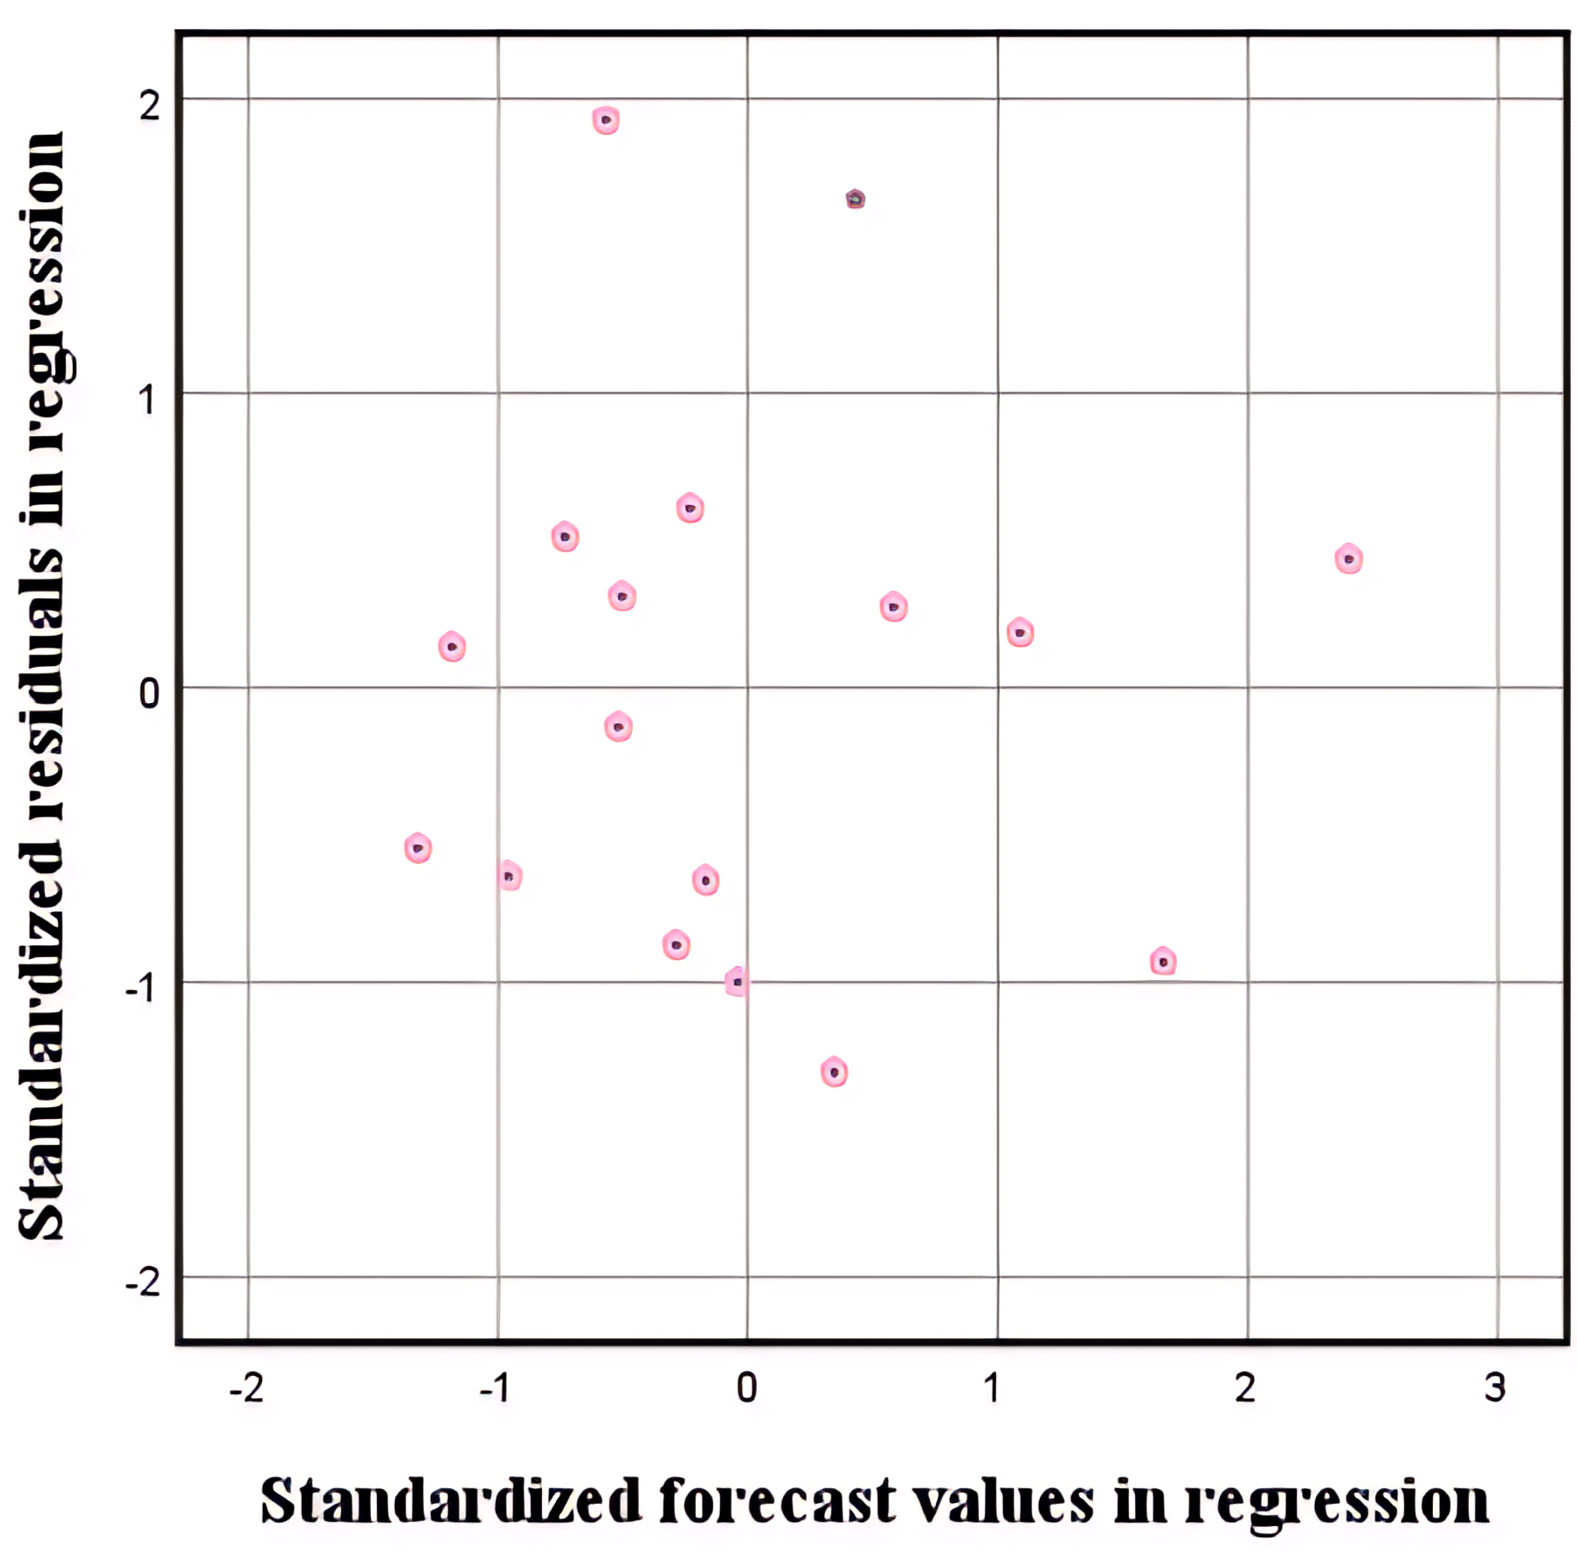
\includegraphics[width=1\linewidth]{Residual plot.png}
		\caption{Residual plot}
	\end{minipage}
	\begin{minipage}{0.4\linewidth}
		\centering
		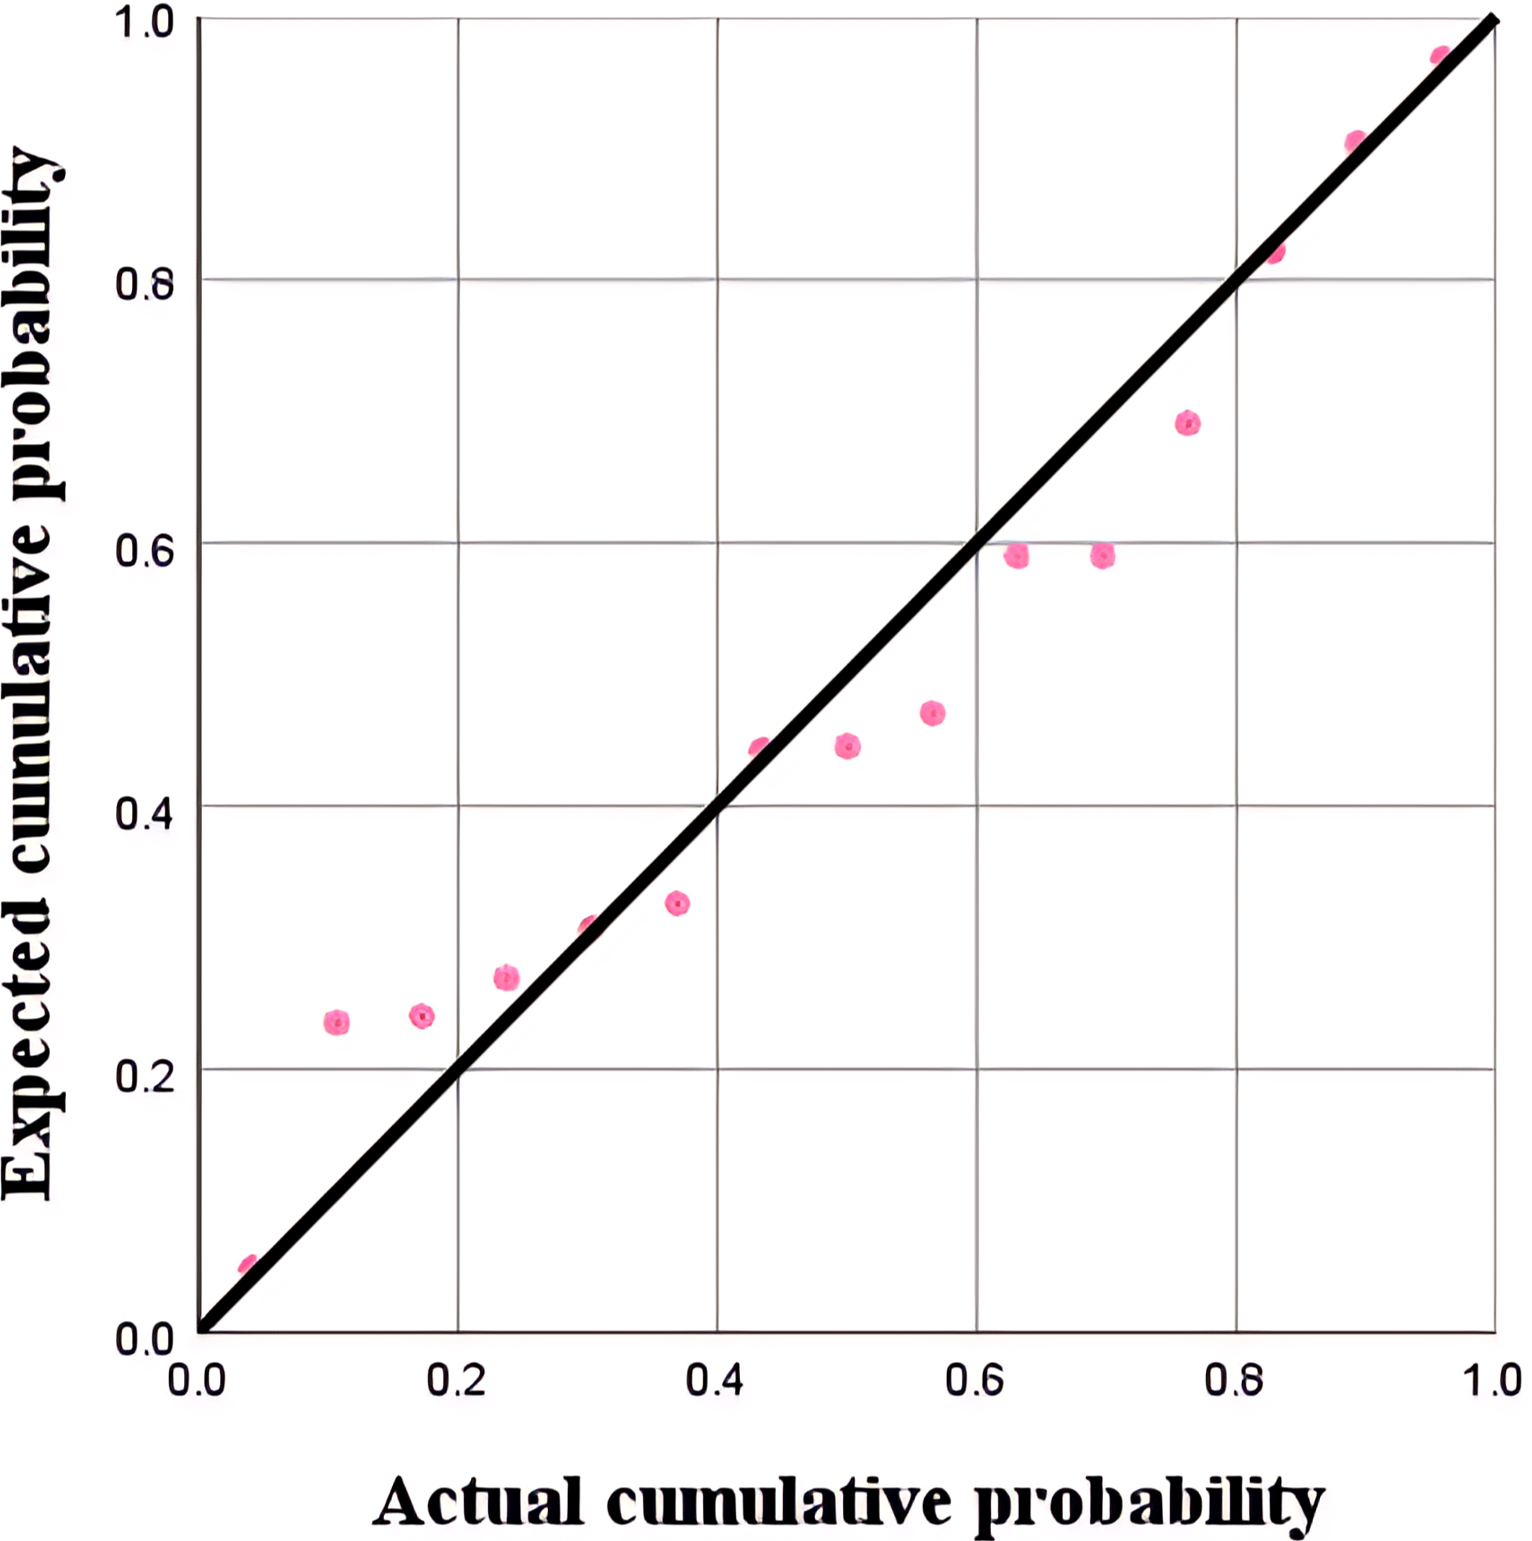
\includegraphics[width=1\linewidth]{Quantile-Quantile Plot.png}
		\caption{Quantile-Quantile plot}
	\end{minipage}
\end{figure}

From the above residual plot and Quantile-Quantile plot, we can see that the residuals are evenly distributed around the horizontal axis, indicating that there is no heteroscedasticity. Additionally, the Quantile-Quantile plot is mostly close to the straight line, which implies that the predictions regarding cumulative probabilities made by this model are fairly accurate overall. This means that the model is capable of capturing the distribution characteristics of the data to some extent, demonstrating a degree of reasonableness and effectiveness.

\subsection{Revealing the results of the medal table for future Olympic Games}
\subsubsection{Analysis of Prediction Model Results}
Based on the modified multiple linear regression trend prediction model, we have obtained the medal-winning trends of participating countries since 1986, excluding those countries that did not hold the Olympics normally, including countries that have never won a medal. The regression results for all participating countries have been obtained, and we will now list the regression results for some countries in the table below:

\begin{table}
\centering
\caption{Regression coefficient of the trend prediction model}
\begin{tabular}{|c|c|c|c|c|c|c|} 
\hline
\multirow{2}{*}{Country} & \multicolumn{5}{c|}{$\theta$}               & \multirow{2}{*}{$R^{2}$}  \\ 
\cline{2-6}
                         & a1    & a2    & a3    & a4    & a5    &                    \\ 
\hline
Australia                & 0.023 & 0.141 & 0.190 & 0.351 & 0.281 & 0.877              \\ 
\hline
Belarus                  & 0.011 & 0.054 & 0.113 & 0.000 & 0.764 & 0.769              \\ 
\hline
Belgium                  & 0.124 & 0.314 & 0.215 & 0.241 & 0.465 & 0.864              \\ 
\hline
China                    & 0.141 & 0.521 & 0.121 & 0.327 & 0.684 & 0.880              \\ 
\hline
United States            & 0.118 & 0.381 & 0.241 & 0.261 & 0.763 & 0.792              \\
\hline
\end{tabular}
\end{table}

The estimated regression coefficients shown in the above table reflect the number and types of events in which each country participates, the overall performance of athletes in each country measured by the number of medals won, as well as a quantitative analysis of the past winning situations and the host country effect based on historical data. The regression results indicate that these factors positively influence the medal-winning rates of the countries.
Next, we estimated the probability of each country winning gold medals using a modified Bayesian model, continually refining the probabilities with existing data to achieve optimal estimation results.

Based on historical data, assuming that the number and types of events as well as the performance levels of participating athletes in each country remain stable, and knowing that the host country is the United States with past winning situations for 2024, we predict the medal tally for the 2028 Los Angeles Summer Olympics. Additionally, we provide the prediction intervals with a confidence level of 0.95 for all countries, as shown in Table 5:

\begin{table}
\centering
\caption{Prediction interval for the number of Medalsa in difference Country}
\arrayrulecolor[rgb]{1,0.482,0}
\begin{tabular}{|c|ccc|} 
\hhline{|----|}
\rowcolor[rgb]{1,0.482,0} \multicolumn{1}{|c}{{\cellcolor[rgb]{1,0.482,0}}}                                      & {\cellcolor[rgb]{1,0.482,0}}                                    & \multicolumn{2}{c|}{~ ~Confidence interval of 0.95~ ~}                             \\
\rowcolor[rgb]{1,0.482,0} \multicolumn{1}{|c}{\multirow{-2}{*}{{\cellcolor[rgb]{1,0.482,0}}~ ~ ~ Country~ ~ ~~}} & \multirow{-2}{*}{{\cellcolor[rgb]{1,0.482,0}}~ ~ Pre\_2028~ ~~} & {\cellcolor[rgb]{1,0.824,0.635}}LMCI\_2 & {\cellcolor[rgb]{1,0.824,0.635}}UMCI\_2  \\ 
\hline
{\cellcolor[rgb]{0.992,0.737,0.529}}United States                                                                & 106                                                             & 94                                      & 134                                      \\ 
\hline
\rowcolor[rgb]{1,0.824,0.635} {\cellcolor[rgb]{0.992,0.737,0.529}}China                                          & 87                                                              & 72                                      & 102                                      \\ 
\hline
{\cellcolor[rgb]{0.992,0.737,0.529}}GreatBritain                                                                 & 82                                                              & 41                                      & 123                                      \\ 
\hline
\rowcolor[rgb]{1,0.824,0.635} {\cellcolor[rgb]{0.992,0.737,0.529}}Germany                                        & 59                                                              & 37                                      & 80                                       \\ 
\hline
{\cellcolor[rgb]{0.992,0.737,0.529}}Australia                                                                    & 47                                                              & 37                                      & 57                                       \\ 
\hline
\rowcolor[rgb]{1,0.824,0.635} {\cellcolor[rgb]{0.992,0.737,0.529}}Italy                                          & 42                                                              & 30                                      & 55                                       \\ 
\hline
{\cellcolor[rgb]{0.992,0.737,0.529}}Japan                                                                        & 42                                                              & 33                                      & 51                                       \\ 
\hline
\rowcolor[rgb]{1,0.824,0.635} {\cellcolor[rgb]{0.992,0.737,0.529}}SouthKorea                                     & 35                                                              & 22                                      & 48                                       \\ 
\hline
{\cellcolor[rgb]{0.992,0.737,0.529}}Netherlands                                                                  & 27                                                              & 19                                      & 36                                       \\ 
\hline
\rowcolor[rgb]{1,0.824,0.635} {\cellcolor[rgb]{0.992,0.737,0.529}}France                                         & 23                                                              & -4                                      & 51                                       \\ 
\hline
{\cellcolor[rgb]{0.992,0.737,0.529}}Hungary                                                                      & 23                                                              & 15                                      & 32                                       \\ 
\hline
\rowcolor[rgb]{1,0.824,0.635} {\cellcolor[rgb]{0.992,0.737,0.529}}Cuba                                           & 22                                                              & 13                                      & 32                                       \\ 
\hline
{\cellcolor[rgb]{0.992,0.737,0.529}}Canada                                                                       & 20                                                              & 12                                      & 28                                       \\ 
\hline
\rowcolor[rgb]{1,0.824,0.635} {\cellcolor[rgb]{0.992,0.737,0.529}}Ukraine                                        & 19                                                              & 4                                       & 33                                       \\ 
\hline
{\cellcolor[rgb]{0.992,0.737,0.529}}Brazil                                                                       & 18                                                              & 15                                      & 22                                       \\ 
\hline
\rowcolor[rgb]{1,0.824,0.635} {\cellcolor[rgb]{0.992,0.737,0.529}}Spain                                          & 18                                                              & 5                                       & 31                                       \\ 
\hline
{\cellcolor[rgb]{0.992,0.737,0.529}}Sweden                                                                       & 16                                                              & 7                                       & 26                                       \\ 
\hline
\rowcolor[rgb]{1,0.824,0.635} {\cellcolor[rgb]{0.992,0.737,0.529}}Kenya                                          & 15                                                              & 9                                       & 21                                       \\ 
\hline
{\cellcolor[rgb]{0.992,0.737,0.529}}Norway                                                                       & 15                                                              & 8                                       & 21                                       \\ 
\hline
\rowcolor[rgb]{1,0.824,0.635} {\cellcolor[rgb]{0.992,0.737,0.529}}Poland                                         & 15                                                              & 8                                       & 22                                       \\
\hline
\end{tabular}
\arrayrulecolor{black}
\end{table}

From the changes in the number of medals won by various countries, the ten countries with the most significant changes are the United Kingdom, Norway, New Zealand, the Netherlands, Iran, Canada, Uzbekistan, Cuba, Germany, and France. The changing trends are illustrated in Figure XXX:

\begin{figure}[h] 
\centering
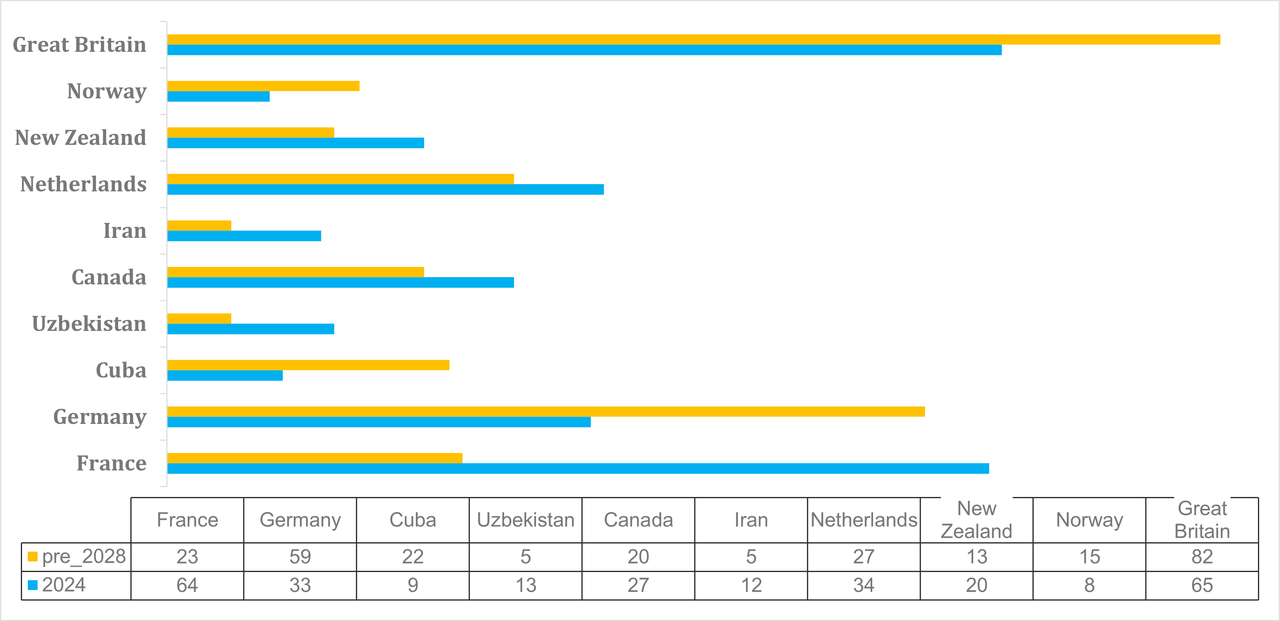
\includegraphics[width=10cm]{Chart of the Medal Counts Changes of the Top 10 Countries.png}
\caption{Chart of the Medal Counts Changes of the Top 10 Countries}
\end{figure}

Analyzing the figure, it can be concluded that the countries predicted to see significant improvements in their medal counts include Germany, Cuba, Norway, and the United Kingdom. Conversely, the countries with declining results should not be overlooked, notably France, Uzbekistan, Canada, Iran, the Netherlands, and New Zealand. Specifically, compared to 2024, it is expected that France will see a reduction of 41 medals in 2028, which warrants attention.

Regarding the changes in rankings among countries, the ten countries with the most significant ranking changes are the Philippines, Cuba, Poland, Slovenia, Austria, Iran, Kyrgyzstan, Turkey, Uzbekistan, and Ireland. The changing trends are illustrated in Figure 11:

\begin{figure}[h] 
\centering
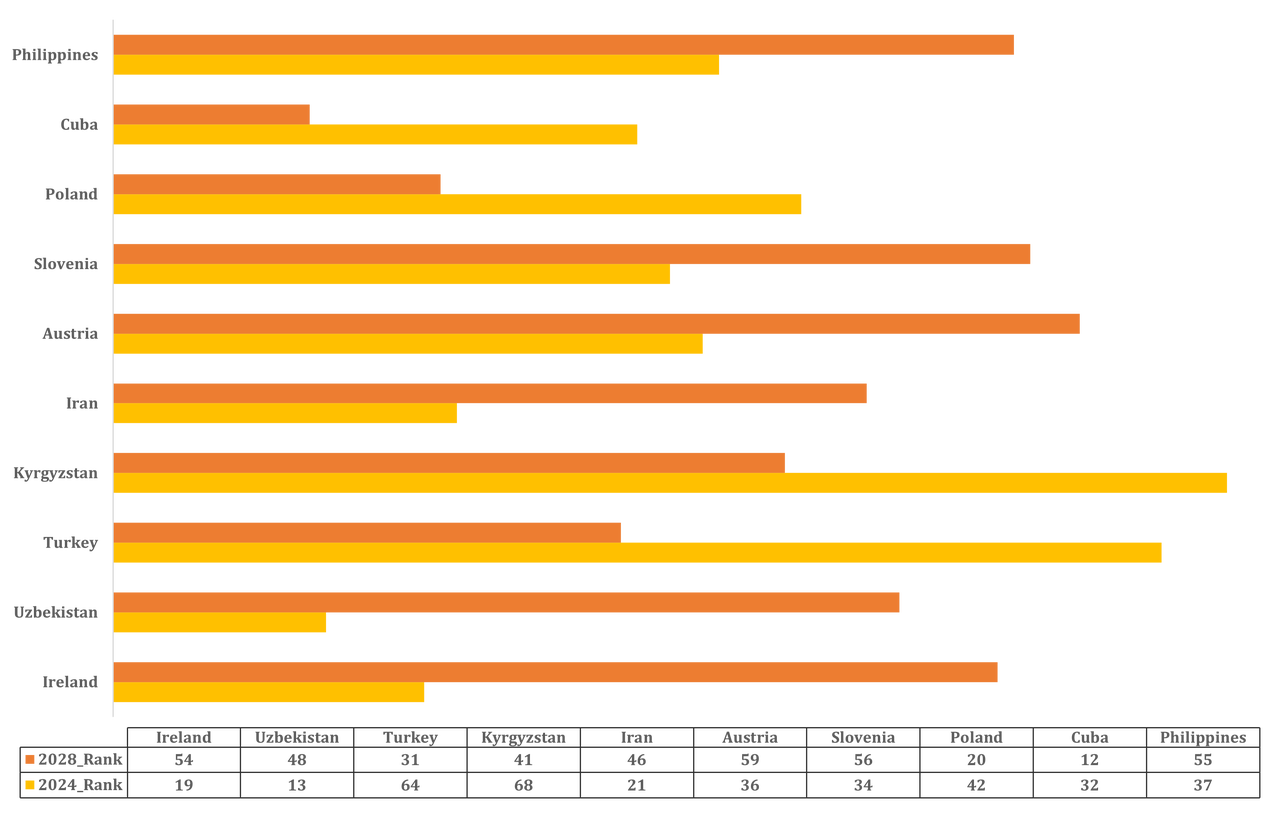
\includegraphics[width=10cm]{Chart for Comparing the Ranking Changes of the Top 10 Countries.png}
\caption{Chart for Comparing the Ranking Changes of the Top 10 Countries}
\end{figure}

Analyzing the figure, it can be observed that the countries with significant improvements in their rankings include Turkey, Kyrgyzstan, Poland, and Cuba. Furthermore, it is predicted that the rankings of the Philippines, Slovenia, Austria, Iran, Uzbekistan, and Ireland will decline significantly. Notably, both Ireland and Uzbekistan are projected to drop 35 positions, marking the most pronounced changes in rankings.

The calculations regarding the likelihood of countries that have never won a medal obtaining their first medal at the 2028 Olympics, along with the corresponding estimated probabilities, are shown in Table 6.

\begin{table}
\centering
\caption{Table of the Countries Achieving Zero-breakthrough and  Probabilities}
\begin{tabular}{|c|c|c|c|} 
\hline
\textbf{~ ~ ~ Country~ ~ ~~} & \textbf{~ Probability~~} & \textbf{Country}                 & \textbf{~ Probability~~}  \\ 
\hline
Nicaragua                    & 0.129217                 & Tuvalu                           & 0.131417                  \\ 
\hline
Libya                        & 0.112495                 & South Sudan                      & 0.118437                  \\ 
\hline
Comoros                      & 0.144345                 & Lebanon                          & 0.131196                  \\ 
\hline
Malawi                       & 0.130465                 & Democratic Republic of the Congo & 0.145907                  \\ 
\hline
Rhodesia                     & 0.131206                 & East Timor                       & 0.102365                  \\ 
\hline
Cook Islands                 & 0.100384                 & Eswatini                         & 0.097714                  \\ 
\hline
Peri                         & 0.137529                 & St Kitts and Nevis               & 0.116556                  \\ 
\hline
South Vietnam                & 0.140657                 & StVincentGrenadines              & 0.122315                  \\ 
\hline
Cambodia                     & 0.148522                 & Timor-Leste                      & 0.13819                   \\ 
\hline
Kingfisher                   & 0.117098                 & Brunei Darussalam                & 0.097726                  \\ 
\hline
Yangon                       & 0.129572                 & DR Congo                         & 0.120408                  \\
\hline
\end{tabular}
\end{table}

After processing and analyzing the data, it was found that since the first Olympic Games in 1886, a total of 101 countries have never won a medal based on historical participation data. Among these countries, some are temporary teams, some have ceased to exist due to historical reasons, and others have failed to participate continuously due to special circumstances. This paper does not consider these special situations or distinguish among these countries, but rather focuses on their participation records and medal-winning situations.

Assuming these countries continue to participate in the 2028 Olympics, we used a multiple linear regression model to predict their medal-winning outcomes. The results indicate that 22 countries are likely to achieve a “breakthrough” in winning their first medal in history during the 2028 Olympics. However, the predicted probabilities of winning vary among the countries and are relatively low. This is largely due to the analysis of their past performance at previous Olympics and the lack of prominent competitive advantages in their events.

Considering the wide range of events included in the Olympics, which not only have numerous categories but also encompass everything from physically demanding sports like athletics and swimming to skill-based events like gymnastics and diving, as well as team sports such as basketball and football, an in-depth analysis of medal predictions reveals significant disparities in strength across different Olympic disciplines.

For instance, the United States showcases an absolute advantage in many events. Given this strong performance in favored events, continuing to invest in these areas is undoubtedly a key strategy to maintain its leading position in the Olympic medal table. However, for more balanced events, such as badminton, where the overall strength of the U.S. still has room for improvement compared to traditional strong teams in Asia, more investment should be made to elevate performance. In disadvantageous events, such as archery, the significant gap between the United States and archery powerhouses like Korea and China indicates the need for continuous efforts to enhance capabilities and overcome the disadvantages.

\section{Task 2}
\subsection{Great Coach Effect}

The Great Coach Effect refers to the positive impact that an outstanding coach has on a team or individual athletes. This effect encompasses various aspects, including improved athlete performance, enhanced team cohesion, and increased personal skills and tactical understanding. When Lang Ping coached the Chinese women's volleyball team, she created opportunities for each player to showcase their potential and unleash their energy. Bela Karolyi not only focused on improving athletes' skills but also emphasized the cultivation of their mental resilience, ensuring they could perform consistently well in critical moments.

Through the review and study of literature, we found that coaches play a crucial role in enhancing athletes' performance levels. According to the analysis results from Model One, the level of athletes is a core factor determining a country's medal-winning outcomes at the Olympics. It is evident that coaches have a direct influence on athlete performance, which in turn indirectly affects a country's Olympic performance—specifically, the number of medals won.
To further explore the impact of the Great Coach Effect on the number of medals, we will focus on the direct effect as our entry point. First, we will analyze the direct influence of coaches on athlete performance. After clarifying this influence mechanism, we will use the model established in the first question to further deduce the impact of coaches on their country's medal count. This research approach will help us to gain a more comprehensive and in-depth understanding of the key role coaches play in their nation's Olympic achievements.

\begin{figure}[h] 
\centering
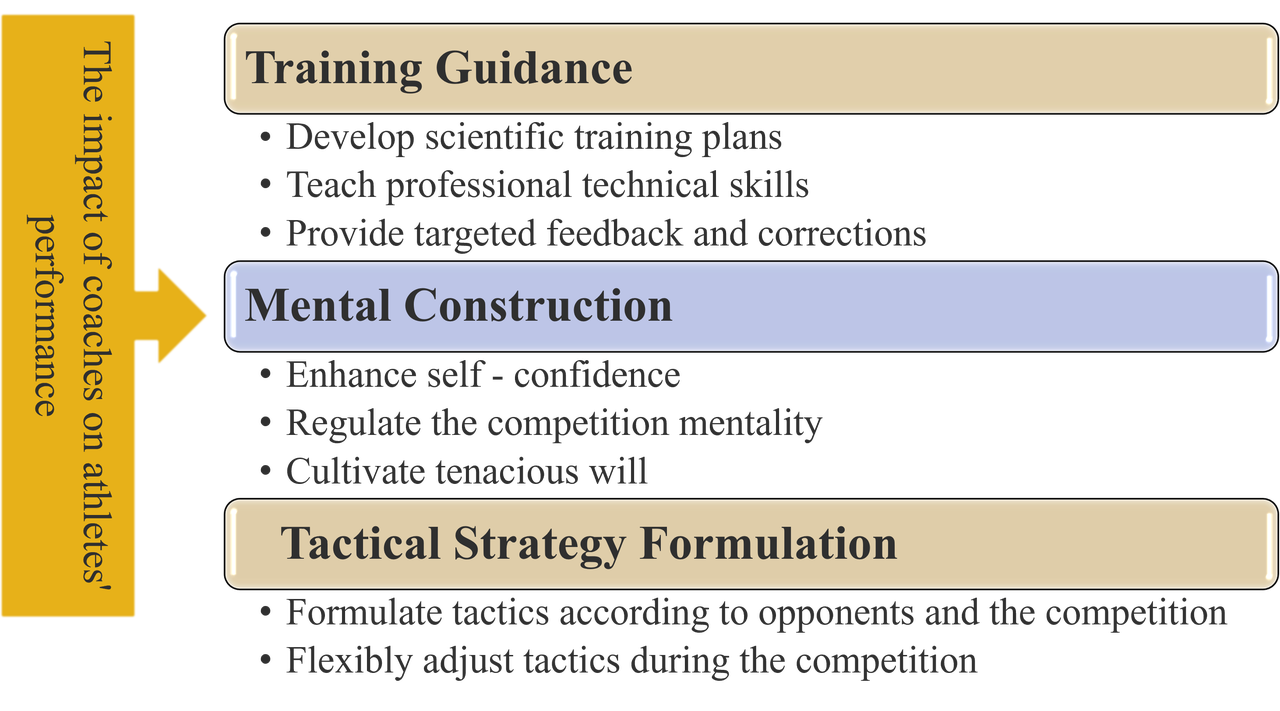
\includegraphics[width=8cm]{The impact of coaches on athletes' performance.png}
\caption{The impact of coaches on athletes' performance}
\end{figure}

\subsection{Qualitative Analysis}
\hskip\parindent The Károlyi gym, established by Márta Károlyi in the late 1980s, has become an exceptional training facility in the United States. Following this development, we can observe a significant increase in the average number of medals won by the U.S. women's gymnastics team, with 1980 serving as a pivotal dividing line.

\begin{figure}[h] 
\centering
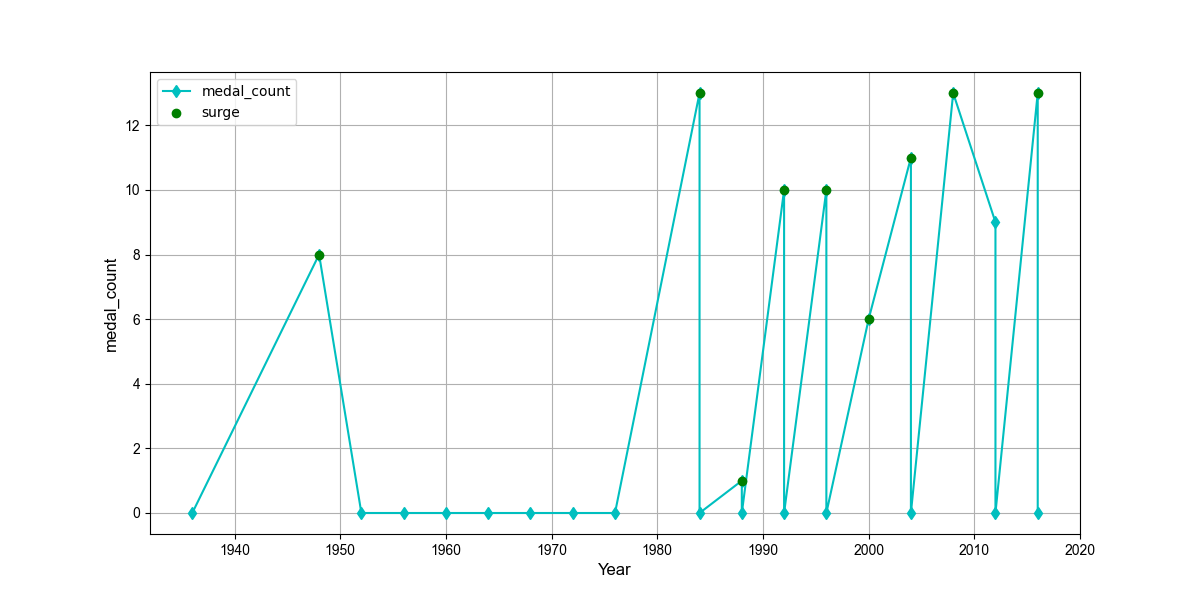
\includegraphics[width=8cm]{The number of Olympic medals won by the United States in women's gymnastics.png}
\caption{The number of Olympic medals won by the United States in women's gymnastics}
\end{figure}

The transition from having no gold medals to winning them can be clearly observed in the chart below. Prior to 1980, the United States had not won any Olympic gold medals in women's gymnastics. However, after 1980, the number of gold medals won increased significantly, not just by one or two, but rather by a remarkable surge.

\begin{figure}[h] 
\centering
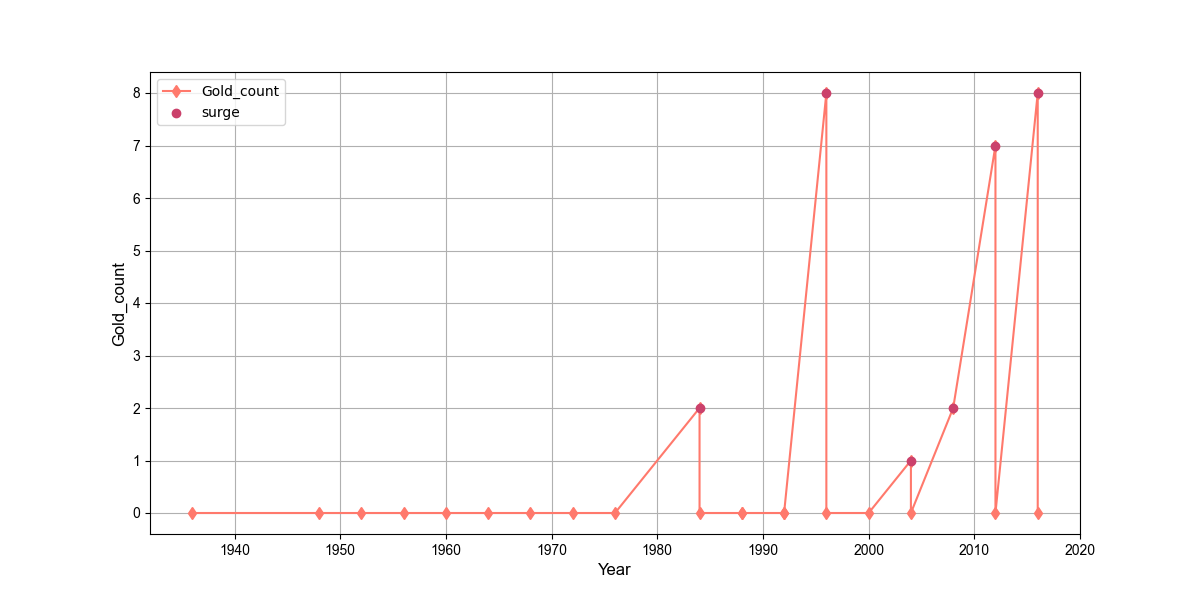
\includegraphics[width=8cm]{The number of Olympic gold medals won by the United States in women's gymnastics.png}
\caption{The number of Olympic gold medals won by the United States in women's gymnastics}
\end{figure}

By comparing the historical medal counts for women's volleyball in China and the United States, we can identify two key focal points in time. The first is 1995, when Lang Ping became the head coach of the Chinese national team, leading them from a period of decline to success. The second point is in 2008, when Lang Ping took over as head coach of the U.S. team, which had gone three consecutive years without winning any medals. Under her guidance, the team not only secured medals but also maintained their success for two consecutive years.

\begin{figure}[h] 
\centering
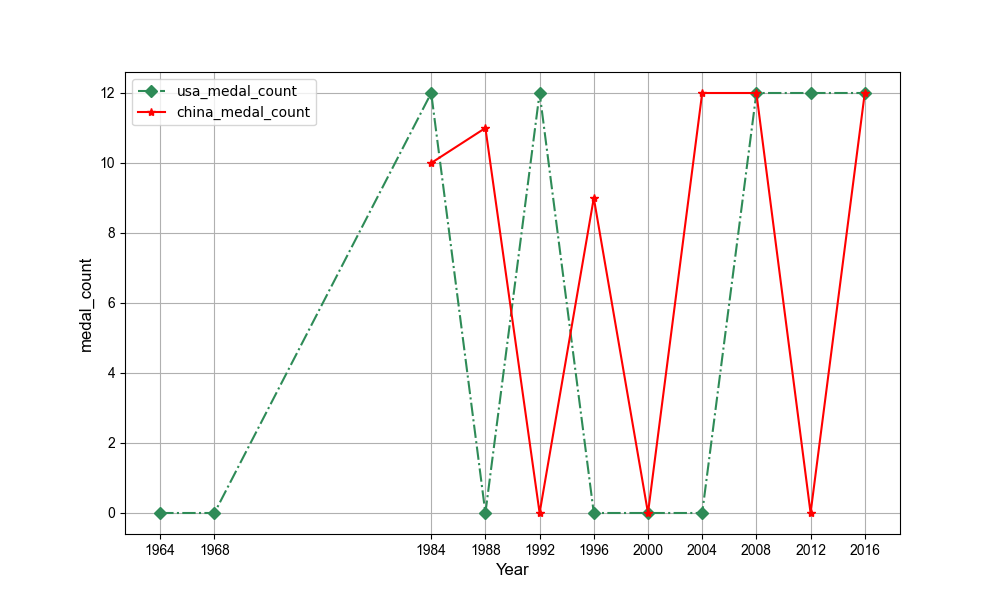
\includegraphics[width=8cm]{The number of Olympic medals won by China and the United States in women's volleyball.png}
\caption{The number of Olympic medals won by China and the United States in women's volleyball}
\end{figure}

To further analyze the impact of outstanding coaching effects on the number of medals, a one-sample Wilcoxon signed-rank test was conducted on the above data. Some of the results are as follows:

\begin{table}[h]
\centering
\caption{Table of variance analysis}
\begin{tabular}{|c|c|c|c|c|} 
\hline
\textcolor[rgb]{0.031,0.031,0.031}{~ Inspection value~~} & \textcolor[rgb]{0.031,0.031,0.031}{~ ~ Sample size~ ~~} & \textcolor[rgb]{0.031,0.031,0.031}{Standard deviation} & ~ z~~ & P        \\ 
\hline
1.12                                                     & 25                                                      & 2.538                                                  & 2.43  & 0.015**  \\ 
\hline
2.34                                                     & 25                                                      & 2.349                                                  & 3.26  & 0.011**  \\ 
\hline
2.12                                                     & 24                                                      & 1.956                                                  & 2.81  & 0.019**  \\
\hline
\end{tabular}
\end{table}

Based on the variable Medal_count in U.S. gymnastics and its mean of 1.12, the significance P-value is 0.015, which is less than 0.05, indicating statistical significance. Therefore, we reject the null hypothesis, suggesting that there is a significant difference in award outcomes before and after the introduction of coaching. Similarly, for other sports, there are also significant differences in award outcomes before and after the introduction of outstanding coaches.

\subsection{Quantitative analysis}
First, we quantify the performance level of athletes from this country by calculating the medal-winning rate for all athletes in their respective events. The formula for this calculation is:

\begin{equation}
P_{i, j}(t) = M_{i, j}(t) / S_{i, j}(t)
\end{equation}

Where, $P_{i, j}(t)$ represents the medal-winning rate of country $i$ in event $j$ at the Olympic Games in year $t$; $M_{i, j}(t)$ indicates the number of medals won by country $i$ in event $j$ at the Olympic Games in year $t$ (counted by the number of medals, not by events); and $S_{i, j}(t)$ represents the total number of athletes from country $i$ participating in event $j$ at the Olympic Games in year $t$.

Then, $\Delta P_{i, j} = P_{i, j}(t_{1}) - P_{i, j}(t_{0})$ represents the change in the performance level of country $i$'s athletes in event $j$ from the Olympic Games in year $t0$ to the Olympic Games in year $t1$. Furthermore, assuming that the coach started coaching in a certain year $t0$, we can quantify the impact of the coach on athletes' performance levels by comparing the average changes in athlete performance level before and after the coach's arrival:

\begin{equation}
\Delta P_{i, j} = \bar{P}_{i, j}^{after}(t_{0}) - \bar{P}_{i, j}^{before}(t_{0})
\end{equation}

Where, $\bar{P}_{i, j}^{after}(t_{0})$ represents the average performance level of country $i$'s athletes in event $j$ after the coach's arrival; $\bar{P}_{i, j}^{before}(t_{0})$ represents the average performance level of country $i$'s athletes in event $j$ before the coach's arrival. Thus, the impact of the coach on the total number of medals can be expressed as:

\begin{equation}
\Delta M_{i, j}(t) = \Delta P_{i, j} \times A_{i, j}(t)
\end{equation}

Where, $\Delta M_{i, j}(t)$ represents the number of additional medals won by country $i$ in event $j$ at the Olympic Games in year $t$ after the coach's arrival.

Based on the available data, it can be calculated that for the United States in gymnastics, the quantified performance level of athletes before Márta Károlyi's coaching was 0.3125. After he became the coach, the athletes' performance level clearly improved in the subsequent Olympic Games, reaching 0.751. Similarly, for China in volleyball, before Lang Ping's coaching, the team had been at a disadvantage, with a quantified athlete performance level of only 0.1756. After Lang Ping took over as coach in 1995, China's quantified athlete performance level increased to 0.751. This further validates that the influence of coaches on athlete performance levels is profound.

\subsection{Investment in Excellent Coaches Based on Benefit Analysis}
The impact and significance of the Olympics on various countries are profound, serving not only as a key window to showcase athletic strength but also as a powerful booster for enhancing international image. Therefore, investing in great coaching programs holds significant and irreplaceable value, yielding multifaceted returns. Through scientific training methods, excellent coaches are always able to significantly enhance the overall performance of athletes and teams, thereby bringing high returns and efficiencies to their countries.

Based on the analysis of the medal standings for the United States at the 2028 Los Angeles Summer Olympics in the first question, an analysis of the medal outcomes for the 2024-2028 Olympics revealed that Ireland, Uzbekistan, and Iran ranked high in the 2024 medal standings. However, their predicted performances in the 2028 standings do not look optimistic. This prediction undoubtedly serves as a wake-up call for these three countries. Given the multiple profound impacts of the Olympics on nations, it is highly probable that these countries will take a series of strong measures to enhance their athletes' competitive levels.

Therefore, this paper chooses these three countries, which ranked among the top yet are predicted to see a significant decline in performance compared to 2024, for analysis. Further analysis of their respective strong, balanced, and weak events is detailed in the table below:

\begin{table}
\centering
\caption{Description of the Advantages and Disadvantages of Events}
\begin{tabular}{|c|c|c|} 
\hline
\textbf{~ NOC~~}     & \textbf{~ ~ A\_Sport~ ~~} & \textbf{~ ~ ~B\_Sport~ ~~}  \\ 
\hline
\multirow{2}{*}{IRL} & Aquatics                  & Boxing                      \\ 
\cline{2-3}
                     & Athletics                 & Rowing                      \\ 
\hline
\multirow{2}{*}{UZB} & Boxing                    & Gymnastics                  \\ 
\cline{2-3}
                     & Taekwondo                 & Judo                        \\ 
\hline
\multirow{3}{*}{IRI} & Karate                    & Athletics                   \\ 
\cline{2-3}
                     & Shooting                  & Weightlifting               \\ 
\cline{2-3}
                     & Taekwondo                 & Wrestling                   \\
\hline
\end{tabular}
\end{table}

Through the mining of the existing dataset, it is found that for Ireland, the strong events are Aquatics, Athletics, and Gymnastics, whereas Boxing and Rowing are the weak events; other events can be considered the balanced events for the country. For Uzbekistan, the strong events are Boxing, Taekwondo, and Weightlifting, while Gymnastics and Judo are the weak events. For Iran, the strong events are Karate, Shooting, and Taekwondo, while Athletics and Weightlifting are identified as the weak events.

From the quantitative analysis results of the effects of excellent coaches, it is evident that after the introduction of excellent coaches, the competitive level of athletes in these events will improve to a certain extent, denoted as $\Delta P_{i, j}$.

\begin{equation}
MP^{i} = a_{1} ^ {i} + a_{2} ^{i}\times S_{1}\_Num^{i} + a_{3}^{i}\times P_{1}\_Num^{i} + a_{5}^{i}M
\end{equation}

Where, $P_{1}\_Num^{i}=P_{ij} + \Delta P_{i, j} + P\_Num^{i}$; $M$ represents the historical number of gold medals won.

We use the following formula to estimate the impact of investment in the great coaching program on the increase in the number of medals won:

\begin{equation}
\Delta M=M_{c} - M_{b}
\end{equation}

Where, $\Delta M$ represents the additional number of medals obtained after the introduction of excellent coaches; $M_{c}$ refers to the predicted number of medals won after the introduction of excellent coaches; and $M_{b}$ denotes the number of medals won without the introduction of excellent coaches.

Thus, $\Delta M$ is the increase in the number of medals attributable to the investment in the excellent coaching program for these three countries.

\section{Task 3}

\subsection{Preliminary Analysis}
In the early years of the Olympics, the participation rate of women was extremely low. However, in recent years, with the advancement of civilization, women have gradually begun to emerge in the Olympic Games. The proportion of female participants in the total participation records has steadily increased, and by the 2024 Olympics, the participation rate of women is expected to be on par with that of men.

The majority of participants did not win any medals: 78.67\% of individuals (102,269 people) did not receive any medals. This observation reveals a clear Pareto effect, where 80\% of the medals are concentrated among 20\% of the participants, indicating that the vast majority of Olympic participants did not secure any medals.

A minority of individuals won medals: only 16.12\% of participants (20,957 people) earned one medal, while 3.50\% (4,546 people) won two medals. This demonstrates that the number of medal winners is relatively small, and the count decreases rapidly as the number of medals increases.

Sparsity of medal distribution: As the number of medals increases, the number of individuals who win medals decreases significantly. Only 0.14\% of participants (187 people) won five medals, and 0.09\% (113 people) won six medals, with the number of winners declining sharply after three medals.

A very small number of individuals achieved a high medal count: the data indicates that the number of participants who won ten or more medals is exceedingly rare, with only 17 individuals winning ten medals, and just one person winning 18 and 28 medals, respectively. This suggests that instances of winning a high number of medals are extremely uncommon within this dataset.

Distribution skewness: Overall, this distribution exhibits a pronounced positive skewness, indicating that the majority of individuals cluster around low medal counts (0-2 medals), while the distribution of higher medal counts is relatively sparse.

\begin{figure}[H] 
\centering
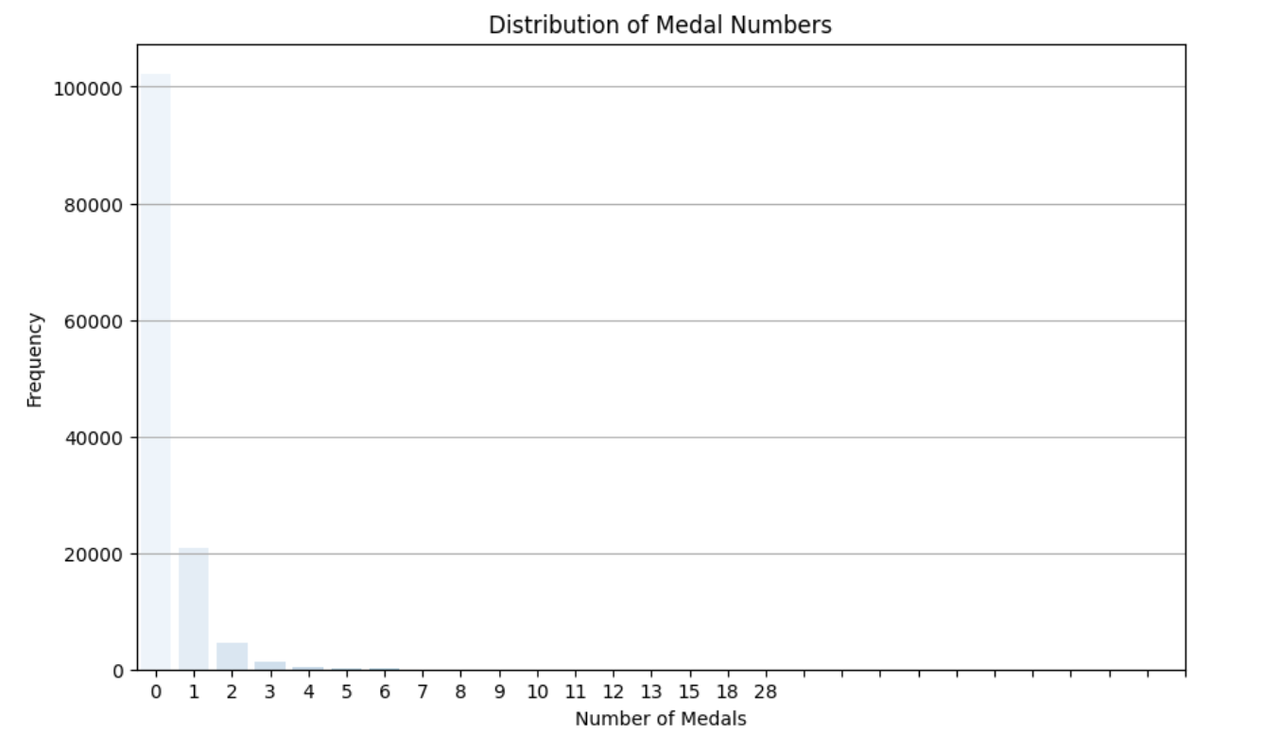
\includegraphics[width=12cm]{The changing participation rate of female athletes in various Olympic Games.png}
\caption{The changing participation rate of female athletes in various Olympic Games}
\end{figure}

We also observe that certain events are dominated by specific countries in terms of medal acquisition. For instance, countries such as the USA (Roque), SUI (Aeronautics), FRA (Croquet), GBR (Racquets), and ESP (Basque Pelota) have achieved a 100\% medal share in their respective sports events, indicating that these nations possess an absolute advantage in these particular competitions.

\begin{table}[H]
\centering
\caption{A descending list of the percentage of medals relative to the total number of medals}
\begin{tabular}{|c|c|c|c|c|} 
\hline
\textbf{~ NOC~~} & \textbf{Sport}        & \textbf{~ medal\_num~~} & \textbf{~ total\_medal\_num~~} & \textbf{~ percentage~~}  \\ 
\hline
USA              & Roque                 & 3                       & 3                              & 100                      \\ 
\hline
SUI              & Aeronautics           & 1                       & 1                              & 100                      \\ 
\hline
FRA              & Croquet               & 8                       & 8                              & 100                      \\ 
\hline
GBR              & Racquets              & 10                      & 10                             & 100                      \\ 
\hline
ESP              & Basque Pelota         & 2                       & 2                              & 100                      \\ 
\hline
GBR              & Cricket               & 21                      & 24                             & 87.5                     \\ 
\hline
GBR              & Motorboating          & 6                       & 7                              & 85.71429                 \\ 
\hline
USA              & Golf                  & 41                      & 58                             & 70.68966                 \\ 
\hline
GBR              & Jeu De Paume          & 2                       & 3                              & 66.66667                 \\ 
\hline
CAN              & Lacrosse              & 36                      & 60                             & 60                       \\ 
\hline
GER              & Alpinism              & 2                       & 4                              & 50                       \\ 
\hline
SUI              & Alpinism              & 2                       & 4                              & 50                       \\ 
\hline
GBR              & Polo                  & 30                      & 65                             & 46.15385                 \\ 
\hline
CHN              & Table Tennis          & 104                     & 228                            & 45.61404                 \\ 
\hline
CHN              & Trampoline Gym        & 5                       & 12                             & 41.66667                 \\ 
\hline
USA              & Ice Hockey            & 11                      & 27                             & 40.74074                 \\ 
\hline
CHN              & Badminton             & 83                      & 216                            & 38.42593                 \\ 
\hline
JPN              & Skateboarding         & 9                       & 24                             & 37.5                     \\ 
\hline
GBR              & Figure Skating        & 10                      & 27                             & 37.03704                 \\ 
\hline
CHN              & Trampolining          & 11                      & 30                             & 36.66667                 \\ 
\hline
SUI              & Cycling Mountain Bike & 4                       & 11                             & 36.36364                 \\
\hline
\end{tabular}
\end{table}
Additionally, there is a notable number of countries and events with moderate medal shares. For instance, CAN (Lacrosse) and GER, SUI (Alpinism) have medal shares ranging from 50\% to 60\%, demonstrating a certain level of competitiveness, although they do not reach a monopolistic status. Similarly, CHN (Table Tennis) and CHN (Badminton) account for 45.61\% and 38.43\% of the medals, respectively, indicating that China also performs strongly in these events.

Furthermore, some countries and events exhibit lower medal shares, such as USA (Ice Hockey) and JPN (Skateboarding), where the medal shares are below 40\%. This suggests that competition in these events is relatively intense, preventing any single nation from establishing a dominant position.


From the above figure, it is evident that the diversification of sports events has a significant positive correlation with the number of Olympic medals obtained. To assess the relationship between the number of medals won by a country and the variety of sports events in which it participates, we employed correlation analysis. The results indicate that the Pearson correlation coefficient between the number of medals and the number of sports events participated in by the country is 0.6228, suggesting a strong positive correlation between the two variables.

\newpage

\subsection{Letter}

\begin{letter}{Enjoy Your Bath Time!}

Subject: Recommendations for Optimizing National Sports Strategy

Dear Leaders of the National Olympic Committee:


\hskip\parindent Following an in-depth analysis of the performance of various countries in international sports events, we have identified several key patterns and data that can provide important guidance for our future sports strategy.

Our analysis of medal distribution characteristics reveals that the vast majority of participants did not win any medals, with 78.67\% of individuals failing to secure a medal, and 80\% of the medals being concentrated among 20\% of the participants. This phenomenon suggests that we should implement measures in two key areas: first, we must acknowledge the Pareto effect and focus on providing enhanced support and resources to those athletes who have already won medals, thereby helping them to achieve continued success in future competitions. Second, we should emphasize the development of emerging athletes, increasing our investment in training new talent, particularly in events where medal counts are currently low, with the aim of achieving breakthroughs in future competitions.

We need to pay particular attention to certain sports. Our analysis indicates that some countries excel in specific events, such as those that completely dominate certain competitions—like the USA (Roque) and SUI (Aeronautics), which have achieved a 100\% medal share in their respective events, demonstrating their absolute advantage. Additionally, countries like GBR (Cricket) and USA (Golf) hold a significant proportion of medals in certain events, showcasing their strong competitiveness. In light of this, we propose three recommendations:
\begin{itemize}
\item We should study the successful experiences of these countries in specific events, analyzing their training methods, resource allocation, and athlete selection criteria, so that we can implement improvements in our corresponding events.
\item Using smaller bathtub if possible
\item Decreasing motions during bath
\item Using bubble bath additives
\item Arranging more faucets of inflow
\end{itemize}

Furthermore, from the perspective of the correlation between the number of medals and the variety of sports events, our analysis indicates a significant positive correlation (Pearson correlation coefficient of 0.62) between the number of medals won by a country and the number of sports events in which it participates. This suggests that increasing the variety of sports events may enhance a country's medal count in international competitions. Therefore, we recommend that, on one hand, we diversify our sports offerings by encouraging athletes to participate in multiple events, particularly in those where we already have a foundational presence, to improve our overall medal count. On the other hand, we should consider allocating resources to support athletes and coaching teams that engage in multiple sports.

We believe that optimizing the national sports strategy, particularly in terms of diversifying sports offerings, rational resource allocation, and nurturing emerging athletes, will significantly enhance our performance in international competitions. We look forward to further discussing these recommendations with you and working together to achieve our goals.

Thank you for your attention and support.

\vspace{\parskip}

Sincerely yours,

Team \# 2517063

\end{letter}

\newpage

\section{Model Sensitivity Analysis}
\subsection{Sensitivity Analysis of Input Parameters}
We conducted a sensitivity analysis on the input parameters of the model established in response to the first question. This analysis aims to test the sensitivity of the predicted number of Olympic medals for a country to variations in the input parameters. Specifically, we performed parameter perturbation experiments by adding Gaussian noise to the model's input parameters. For the variable representing the host country effect, since it has only two possible values (0 or 1), any noise added during the standardization of input data will be directly eliminated. Therefore, we conducted sensitivity analyses on the following factors: total number of events, athlete performance (medal count), and the country's historical medal count. In each parameter analysis, we altered only the specified parameter while keeping the other parameters constant.

The Gaussian noise is defined as follows:

\begin{equation}
p(x)=\frac{1}{\sigma \sqrt{2\pi}}exp(-\frac{(x-\mu)^{2}}{2\sigma ^{2}})
\end{equation}

Where, $x$ represents the amplitude of the random signal; $\mu$ denotes the mean; and $\sigma$ indicates the standard deviation.

Relative error $m_{x} = \frac{\left | Pre_{\_New} - Pre_{\_Old}\right |}{Pre_{\_Old}}\times 100\%$.

Then, we predicted the total number of events in which the country participates, the performance of its athletes, and the historical medal rates, incorporating Gaussian noise along with the host country effect. Specifically, when Gaussian noise was added to the number of events, we independently observed the prediction results for x=21,34,65. When x was set to 21, the relative error reached 8.3\%; when x was set to 34, the relative error increased to 14.3\%; and when x was set to 65, the relative error rose to 18.4\%. Similarly, we tested the performance of athletes and the historical medal rates by adding noise, and the variations in relative error exhibited a certain regularity without any abrupt jumps or anomalous fluctuations. This strongly indicates that the model possesses good adaptability, leading to the conclusion that it is robust in predicting the number of Olympic medals for countries.

\section{Model Evaluation}
\subsection{Strengths}
\begin{itemize}
\item We employed a multiple linear regression model to predict the medal standings, which is easy to understand and interpret. The coefficients of the model directly reflect the extent of influence that each independent variable has on the dependent variable, facilitating the exploration of new independent variables to meet diverse research needs.

\item A significant advantage of our model is its substantial scalability, as it integrates various potential factors into a unified and robust framework, demonstrating effectiveness in predicting future Olympic medals.

\item A significant advantage of our model is its substantial scalability, as it integrates various potential factors into a unified and robust framework, demonstrating effectiveness in predicting future Olympic medals.
\end{itemize}

\subsection{Weaknesses}

\begin{itemize}
\item The presence of high correlation among independent variables may lead to multicollinearity issues, affecting the stability and interpretability of the multiple linear regression model.

\item For the predictions of the medal standings for various countries, the prediction intervals provided by our model are sometimes wider than the actual results. This may result in our model's predictions for these countries being less informative.

\item Due to the limitations in the collection of sample data, some potential influencing factors may not be adequately analyzed, leading to discrepancies between the predicted and actual results.

\item The model makes relatively ideal assumptions about the distribution of the data, which may not hold true in certain cases.
\end{itemize}

\begin{thebibliography}{99}
\addcontentsline{toc}{section}{Reference}

\bibitem{1} Gao Xuan. Analysis of Competitive Performance in Women's Throwing Events in the Last Five Olympic Games and Prediction for the Tokyo Olympic Games [D]. Beijing Sport University, 2018.(In Chinese) 
\bibitem{2} Li Ran. Research on the Competitive Performance of Women's Throwing Events from the 24th to the 32nd Olympic Games and Prediction of the Results for the Paris Olympic Games [D]. Qufu Normal University, 2023. DOI: 10.27267/d.cnki.gqfsu.2023.000828.(In Chinese) 
\bibitem{3} May T P ,Keenan D T ,Potts R , et al.The Sydney 2000 Olympic Games Forecast Demonstration Project: Forecasting, observing network infrastructure, and data processing issues[J].American Meteorological Society,2004,19(1):115-130.
\bibitem{4} Wang Guofan, Zhao Wu, Liu Xujun, et al. Research on Olympic Game Results Prediction Based on GA and Regression Analysis [J]. China Sports Science and Technology, 2011, 47(01): 4-8 + 16. DOI: 10.16470/j.csst.2011.01.002.(In Chinese) 
\bibitem{5} Yang Qinwei. Multivariate Linear Regression Model Predicting the Results of the 2020 Olympic Games [J]. Electronic Production, 2018, (Z2): 121-123. DOI: 10.16589/j.cnki.cn11-3571/tn.2018.z2.058.(In Chinese)
\bibitem{6} Zhang Haibo, Zhao Huancheng. Prediction of the Number of Gold Medals for the Chinese Team in the Beijing Olympic Games [J]. Statistics and Decision, 2008, (15): 76-77. (In Chinese)

\end{thebibliography}

\end{document}
